
%%  ------------------------------------------------------------
%%  DESCRIPTION
%%  ------------------------------------------------------------
%
%  Course material for a basic introduction to R and statistics 
%  4-days long in-house workshop held in April 2010
%  at the Charles Darwin Foundation, Puerto Ayora, Galapagos, Ecuador
%
%  Covers *very* basic but important topics instatistcs and data analysis with R !
%
%%  ------------------------------------------------------------


%  presentation document
\documentclass[mathserif]{beamer}

%%  handout document
 %\documentclass[gray,handout,mathserif]{beamer}

%%  to include only day1, day2, day2 or day3 in the compilation
%  \includeonlylecture{day2}




%% ========================= GENERAL BEAMER THEME OPTIONS ========================= %%{{{
  
%%  modes

%%  presentation mode%%%{{{
\mode<presentation> {
  % ----- complete theme -----
  \usetheme[hideothersubsections]{Hannover}

  % --- inner color theme
  \usecolortheme{rose}

  % ----- uncover behaviour -----
  \setbeamercovered{transparent}
}%%%}}}


%%  handout mode%%{{{
\mode<handout>{
  \usetheme{Pittsburgh}
  \setbeamertemplate{footline}[page number]
  \usepackage{pgfpages}
  \pgfpagesuselayout{4 on 1}[a4paper,border shrink=5mm,landscape]
  \pgfpageslogicalpageoptions{1}{border code=\pgfusepath{stroke}}
  \pgfpageslogicalpageoptions{2}{border code=\pgfusepath{stroke}}
  \pgfpageslogicalpageoptions{3}{border code=\pgfusepath{stroke}}
  \pgfpageslogicalpageoptions{4}{border code=\pgfusepath{stroke}}
  \nofiles
}
%%}}}



% To get rid of navigation symbols at the bottom right of slides
\setbeamertemplate{navigation symbols}{}


% ----- slightly modify the beamer templates -----%%{{{
\setbeamertemplate{blocks}[rounded]
%\setbeamertemplate{enumerate items}[default]%%}}}


% ----- modify colors -----%%{{{
%\setbeamercolor{title}{fg=red!80!black}
%\setbeamercolor{title}{fg=red!80!black,bg=red!20!white}%%%}}}

%%}}}


% ========================= GENERAL CONFIGURATION =========================%%%{{{

% ----- misc layout -----%%{{{
%\setbeameroption{show notes}
%\setbeamertemplate{note page}[compress]
%\urlstyle{sf}%%}}}


% ----- PGF / Tikz graphics -----%%{{{
\usepackage{tikz}
\usetikzlibrary{trees}
\usepgflibrary{arrows}
\usetikzlibrary{arrows}%%}}}


% ----- other options: fonts etc -----%%{{{
\usepackage[spanish,english]{babel}
\usepackage[utf8]{inputenx}


% ----- misc characters (math...) -----%%{{{
\usepackage{ccicons} % icons for Creative Commons
\usepackage{extarrows} % extra arrows
\usepackage{mathabx}   % maths fonts
\usepackage{amsmath}   % maths fonts
\usepackage{wasysym}   % maths fonts
\usepackage{stmaryrd}  % maths fonts
%%}}}


% ----- extra functionalities in arrays -----%%{{{
\usepackage{array}   
\usepackage{multirow}   
%%}}}


% ----- links and pdf -----%%{{{
% cf doc from hyperref for refining options
\hypersetup{%
 colorlinks=true,    %no frame around URL
 urlcolor=olive,    % color  of URLs (brown, gray, 
}%%%}}}


% ----- define command for R logo -----%%{{{
\newcommand{\Rlogo}{
  \protect
\includegraphics[height=2.5ex,keepaspectratio]{figs/Rlogo}
}
%%}}}



% ----- contents at begining of each lecture%%{{{
\AtBeginLecture{%
  \frame{%
  \LARGE %
  \begin{center}
  \structure{\insertlecture}
\end{center} } }
%%}}}


%%% ----- possible contents at begining of each section%%{{{
%  \AtBeginSection[]{%
%    \begin{frame}<beamer| handout:1>{Programa}
%      \tableofcontents[currentsection, hideallsubsections]
%    \end{frame}
%  }
%%%}}}


%%% ----- possible contents at begining of each part%%{{{
%\AtBeginPart{%
% \frame{
%   \partpage
% }
%}
%%%}}}

%%}}}


% ----- TITLE PAGE -----%%{{{
\title[Introducci\'on a la estad\'istica]{Introducci\'on a la estad\'istica}
\subtitle[Bases indispensables y uso de R]{Bases indispensables y uso de \Rlogo}
\author[]{Olivier Devineau}
\institute[]{Fundaci\'on Charles Darwin}
\date[]{Taller interno, 27--30 abril 2010}
%%}}}

%}}}




% ========================= CONTENT =========================%%%{{{
\begin{document}



% ========================= TITLE PAGE [label=title] =========================%%%{{{
\begin{frame}[label=title]
  \titlepage
\end{frame}%%%}}}





% ===== lecture 1 part 1  [label=titlepart1]=====%
\lecture{Introducci\'on y conceptos importantes}{day1}
\part[Introducci\'on]{Introducci\'on y conceptos importantes}



  
% ====================== SECTION: LOGISTICS & CO ======================
\section*{Organizaci\'on del taller}

%  ===== SUBSECTION 1.1: LOGISTICS =====%%%{{{
\subsection*{Log\'istica}

% ----- important stuff [label=admin] -----%%{{{
\begin{frame}[label=admin]
  \frametitle{Cosas importantes}
  \begin{itemize}
    \item Teor\'ia estad\'istica: {\small 8:30--10:00, 10:30--12:00}
    \item Pr\'actica con $R$: {\small 13:30--15:00, 15:30--17:00}
    \item Caf\'e: {\small 10:00--10:30 y 15h00-15h30}
    \item Por favor, apagan los celulares
  \end{itemize}
  \begin{block}{}
    \begin{center}
      ¡Preguntas bienvenidas en cualquier momento!
    \end{center}
  \end{block}
\end{frame}%%}}}
%%}}}


% ===== SUBSECTION 1.2: THANKS =====%%{{{
\subsection*{Agradacimientos}

%----- acknowledgments [label=tnx1] -----%%%{{{
\begin{frame}[label=tnx1]
\frametitle{Agradecimientos}
Use material amablemente provisto por:
  \begin{itemize}
    \item Claude-Pierre Guillaume, \textsc{ephe}, Montpellier, Francia
    \item Damien Caillaud, \textsc{ut}, Austin, Texas, USA
    \item Julien Dutheil, \textsc{cnrs}, Montpellier, Francia
    \item Vladimir Grosbois, \textsc{cirad}, Montpellier, Francia
  \end{itemize}
  \medskip
Correcciones, comentarios y sugerencias por
  \begin{itemize}
     \item Eliana Bontti, \textsc{fcd}
  \end{itemize}
\end{frame}%%}}}

 
% ----- acknowledgments [label=tnx2] ----- %%{{{
\begin{frame}[label=tnx2]
   \frametitle{Agradecimientos}
   Use tambi\'en:
    \begin{itemize}
      \item Crawley, M.J. 2005. \emph{Statistics, an introduction using R.} John Wiley \& Sons.
      \item Quinn, G.P., and Keough, M.J. 2002. \emph{Experimental design and data analysis for biologists.} Cambridge University Press. 
   \end{itemize}
\end{frame}%%}}}
%%}}}








% ================== SECTION: INTRODUCTION: WHAT ARE STATISTICS =============
\section{Introducci\'on}

% ===== SUBSECTION 2.1: WHAT IS IT? =====%%%{{{
\subsection[¿Qu\'e es?]{¿Qu\'e es la estad\'istica?}

%% ----- definition [label=def] -----%%{{{
\begin{frame}[label=def]
  \frametitle{¿Qu\'e es la estad\'istica?}
  \framesubtitle{Definici\'on}
  \begin{itemize}[<+-| handout:1>]
    \item Principios y m\'etodos para recoger, clasificar, resumir y analizar datos 
    \item Aprender, hacer conclusiones y tomar decisiones
  \end{itemize}
\end{frame}%%}}}
%%}}}


% ===== SUBSECTION: WHY ? =====%%{{{
\subsection[La verdadera estad\'istica]{La verdadera estad\'istica}

% ----- example Demostats [label=statsayall]----- %%{{{
\begin{frame}[label=statsayall]
  \frametitle{La verdadera estad\'istica \ldots}
  \framesubtitle{Evoluci\'on de salarios y empleados en una empresa}

    \begin{center}
    \begin{tabular}{lcrrr}
      \hline
                &      & Obreros & Ejecutivos & Promedio \\
      \hline
      Salario   & 2004 &  200    & 2000       & 1100     \\
                & 2006 &  180    & 1800       &  990     \\
      \hline
      Empleados & 2004 & 1000    &  100       &  550     \\
                & 2006 &  600    &  500       &  550     \\
      \hline
    \end{tabular}
    \end{center}

    \medskip 

    \begin{overlayarea}{\textwidth}{3cm}
      \only<2| handout:1>{\begin{description}[==========]
        \item[Peri\'odico] Salarios bajaron en un 10\%
        \item[Empresa] Salario promedio por empleado aument\'o de \$363.6 a \$916.3
      \end{description}%
      }
      \only<3-| handout:1>{\begin{description}[==========]
        \item[Peri\'odico] Hubo despidos en la empresa
        \item[Empresa] Igual n\'umero de empleados y reclutamiento
      \end{description}%
      }
    \end{overlayarea}
\end{frame}
\note[itemize]{
   \item give them some time to make the  calculations and to THINK
   \item los salarios subieron o bajaron?
   \item y el n\'umero the empleados aumento o dismuyo?
   }%%}}}
%%}}}


% ===== SUBSECTION: What can it do ? =====%%%{{{
\subsection[¿Qu\'e puede hacer la esat\'istica?]{¿Que puede hacer la estad\'istica?}

%% ----- what can(not) it do? [label=can-not] -----%%%{{{
\begin{frame}[label=can-not]
   \frametitle{La estad\'istica\ldots}
   \begin{columns}[t, totalwidth=10cm]
   \begin{column}[]{4.8cm}
     \begin{block}{\uncover<1-3| handout:1>{Puede}}<1->
     \begin{itemize}[<1-| uncover@+| handout:1>]
       \item Proveer criterios objetivos para probar hip\'otesis
       \item Optimizar esfuerzos
       \item Evaluar razonamiento de manera cr\'itica
     \end{itemize}
     \end{block}
   \end{column}
   \begin{column}[]{4.8cm}
   \begin{block}{\uncover<4-| handout:1>{\alert{NO} puede}}<1->
     \begin{itemize}[<1-| uncover@+| handout:1>]
       \item Decir la verdad
       \item Compensar ausencia de controles o mala planificaci\'on
       \item Indicar importancia que no es probabil\'istica
     \end{itemize}
   \end{block}
   \end{column}
     \end{columns}
\end{frame}%%%}}}
%%}}}


% ===== SUBSECTION: Descriptive vs inferential =====%%%{{{
\subsection[Descriptiva / inferencial]{Estad\'istica descriptiva y inferencial}

% ----- first step: descriptive [label=desc] -----%%%{{{
\begin{frame}[label=desc]
\frametitle{Primer paso para entender datos: ¡describirlos!}
 \begin{itemize}
   \item Distribuci\'on normal, poisson, binomial \ldots
   \item Media, mediana
   \item Varianza, desviaci\'on est\'andar y error est\'andar
 \end{itemize}
 \medskip
 \hspace{1em} $\Rightarrow$ Estad\'istica \alert{descriptiva} informa sobre forma, centro y amplitud de los datos
\end{frame}%%%}}}


% ----- one step further: inferential [label=infer] -----%%%{{{
\begin{frame}[label=infer]
\frametitle{Describir no es suficiente}
 \begin{itemize}[<1-| uncover@+-| handout:1>]
   \item No es suficiente averiguar que hay variaci\'on
   \item ¿Variaci\'on cient\'ificamente interesante o variaci\'on natural?
\end{itemize}
\bigskip
\onslide+<3-| handout:1>{%
\begin{beamerboxesrounded}[]{Estad\'istica \alert{inferencial} permite:}
  \begin{itemize}
     \item Distinguir entre señal y ruido
     \item Deducir informaci\'on y llegar a conclusiones
  \end{itemize}
\end{beamerboxesrounded}
}%
\end{frame}%%%}}}
%%}}}


% ===== SUBSECTION: Getting started =====%%%{{{
\subsection[¿C\'omo empezar?]{Lo m\'as dif\'icil es empezar}

%% ----- The hardest: getting started [label=getstart] ----- %%{{{
\begin{frame}[label=getstart]
\frametitle{Lo m\'as dif\'icil es empezar}
  \begin{itemize}[<+-| handout:1>]
    \item  ¿Qu\'e tipo de an\'alisis?
    \item Depende de los datos y de la pregunta inicial
    \item  ¿C\'omo saber que hacer? ¡habi\'endolo hecho miles de veces!
  \end{itemize}
\end{frame}%%}}}



% ----- Parametric or not? [label=paramono] ----- %%{{{
\begin{frame}[label=paramono]
\frametitle{¿Estad\'istica param\'etrica o no?}
\begin{columns}[t, totalwidth=10cm]
  \begin{column}[]{4.8cm}
    \begin{block}{\alert{Param\'etrica}}
    \begin{itemize}
      \item Intervalos regulares
      \item Hip\'otesis de distribuci\'on \emph{normal}
      \item Media y error/desviaci\'on est\'andar 
    \end{itemize}
    \end{block}
  \end{column}
  \begin{column}[]{4.8cm}
    \begin{block}{\alert{No param\'etrica}}
    \begin{itemize}
      \item Cualquier tipo de escala
      \item No hip\'otesis de distribuci\'on (independencia)
      \item Mediana y desviaci\'on mediana
    \end{itemize}
    \end{block}
  \end{column}
\end{columns}
\end{frame}%%}}}


% ----- How to start [label=gestart2] ----- %%{{{
\begin{frame}[label=gestart2]
\frametitle{¿Qu\'e preguntarse para empezar?}
 \begin{itemize}[<+-| handout:1>]
   \item ¿Cu\'al es la variable dependiente? 
   \item ¿De qu\'e tipo es? ¿Medida continua, n\'umero, proporci\'on, categor\'ia?
   \item ¿Cu\'ales son las variables independientes? 
   \item ¿Son continuas? ¿Categ\'oricas? ¿Ambos?
\end{itemize}
\end{frame}%%}}}


% -----  Which analysis? (1) [label=whichan1] ----- %%{{{
\begin{frame}[label=whichan1]
\frametitle{¿Qu\'e an\'alisis? Gu\'ia de decisi\'on}
\framesubtitle{1) Variables independientes}
 \begin{itemize}[<+-| handout:1>]
   \item Todas continuas \hfill \alert<.| handout:1>{Regresi\'on}
   \item Todas categ\'oricas \hfill \alert<.| handout:1>{Anova}
   \item Ambas continuas y categ\'oricas \hfill \alert<.| handout:1>{Ancova}
\end{itemize}
\end{frame}%%}}}


% ----- which analysis [label=whichan2] ----- %%{{{
\begin{frame}[label=whichan2]
\frametitle{¿Qu\'e an\'alisis? Gu\'ia de decisi\'on}
\framesubtitle{2) Variable dependiente}
 \begin{itemize}[<+-| handout:1>]
   \item Continua \hfill \alert<.| handout:1>{Regresi\'on normal, Anova, Ancova}
   \item Proporci\'on \hfill \alert<.| handout:1>{Regresi\'on log\'istica}
   \item N\'umero \hfill \alert<.| handout:1>{Regresi\'on log-lineal}
   \item Binaria \hfill \alert<.| handout:1>{An\'alisis log\'istico binario}
   \item Tiempo hasta la muerte \hfill \alert<.| handout:1>{An\'alisis de sobrevivencia}
\end{itemize}
\end{frame}%%%}}}
%%}}}




% ==================== SECTION: variance ===================
\section[Varianza]{Varianza}

% ===== SUBSECTION: Everything varies =====%%{{{
\subsection[Todo varia]{Todo varia}

%% ----- everything varies [label=allvaries] -----%%%{{{
\begin{frame}[label=allvaries]
  \frametitle{Por qu\'e la estad\'istica?}
  \framesubtitle{¡Porque Todo varia!}
  Mucha variabilidad temporal, espacial y entre individuos:
  \begin{itemize}
    \item Gen\'etica
    \item Factores ambientales
    \item Azar
    \item Errores de observaci\'on y medida
  \end{itemize}
\end{frame}%%%}}}
%%}}}


% ===== SUBSECTION: Variance concept =====%%{{{
\subsection[Concepto]{Concepto}
 
% ----- Concept of variance [label=var1] ----- %%{{{
\begin{frame}[label=var1]
   \frametitle{?`Como medir la variabilidad?}
   \vspace{-1cm}
   \begin{columns}[c, totalwidth=10cm]
      \begin{column}[]{5.5cm}
         \flushleft
         \includegraphics<1| handout:0>[scale=0.55]{figs/var1.pdf}
         \includegraphics<2| handout:1>[scale=0.55]{figs/var2.pdf}
         \includegraphics<3-| handout:2->[scale=0.55]{figs/var3.pdf}
      \end{column}
      \begin{column}[]{3.5cm}
         \begin{itemize}
            \item<2-| visible@2-| handout:1-> Rango: $[5,15]$
            \item<3-| visible@3-| handout:2-> Media y desviaciones de la media
            \item<4-| visible@4-| handout:2-> \alert<4>{Residuales}
            \item<5-| visible@5-| handout:2-> $\sum(y-\bar{y}) \only<6->{\alert<6>{=0}}$
            \item<7-| visible@7-| handout:2-> \alert<7>{$SS=\sum(y-\bar{y})^2$}
            \item<8-| visible@8-| handout:2-> \alert<8>{Suma de los cuadrados (sum of squares)}
         \end{itemize}
      \end{column}
   \end{columns}
   \end{frame}%
   \note[itemize]{
      \item  problema del rango: no usa todo los datos y depende demasiado de los valores extremos
   \item cuanto mas largas las lineas de los residuales, lo mas variabilidad hay en los datos
   \item Pero queremos una medida de la variabilidad total. Que tal si hacemos la suma de las longitudes de estas lineas?
   \item no fonctiona porque los residuales de abajo cancelan los de arriba y esta suma es igual a 0 para cualquier nivel de variation
   \item una buena manera de resolver este problema es de usar el cuadrado
   \item cantidad la mas importante de toda la estadistica: suma de los cuadrados o sum of squares en ingles
   }%%}}}


% ----- Mean square deviation [label=var2] ----- %%{{{
\begin{frame}[label=var2]
   \frametitle{Una mejor medida de la variabilidad}
    \begin{itemize}[<+-| visible@+-| handout:1>]
      \item $SS=\sum(y-\bar{y})^2$, $n=11$ 
      \item ?`Que pasa con $SS$ si se agrega un punto?
      \item $SS$ aumenta por cada nuevo punto
      \smallskip
      \item $MS=$\LARGE{$\frac{\sum(y-\bar{y})^2}{\alert<.| handout:1>{n}}$}
      \smallskip
      \item \alert<.| handout:1>{Desviaci\'on cuadr\'atica media} (Mean square deviation $MS$)
   \end{itemize}
\end{frame}%%%}}}
%%}}}


% ===== SUBSECTION: Degrees of freedom =====%%{{{
\subsection[Grados de libertad]{Grados de libertad}

% ----- Degrees of freedom [label=var3] ----- %%{{{
\begin{frame}[label=var3]
   \frametitle{Grados de libertad}
   \begin{itemize}
      \item<1-| visible@1-| handout:1> Muestra de 5 n\'umeros: $\bar{y}=4$ \visible<2->{, $\sum y=20$}
      \smallskip
      \item[] \begin{tikzpicture}
         \visible<1-| handout:1>{\draw (0,0) node[minimum size=1cm,draw] {};
         \draw (1,0) node[minimum size=1cm,draw] {};
         \draw (2,0) node[minimum size=1cm,draw] {};
         \draw (3,0) node[minimum size=1cm,draw] {};
         \visible<1-6| handout:1>{\draw (4,0) node[minimum size=1cm,draw] {}; }}
         \visible<3-| handout:1>{\draw (0,0) node[minimum size=1cm,draw] {2};}
         \visible<4-| handout:1>{\draw (1,0) node[minimum size=1cm,draw] {7};}
         \visible<5-| handout:1>{\draw (2,0) node[minimum size=1cm,draw] {4};}
         \visible<6-| handout:1>{\draw (3,0) node[minimum size=1cm,draw] {0};}
         \visible<7-| handout:1>{\draw (4,0) node[minimum size=1cm,draw,red] {7};}
      \end{tikzpicture}
      \smallskip
      \item<8-| visible@8-| handout:1> Total libertad en la selecci\'on de n\'umeros $1-4$ 
      \item[]<9-| visible@9-| handout:1> $\Rightarrow$ \alert<9>{$4$ grados de libertad} (degrees of freedom \emph{d.f.}\,)
      \item<10-| visible@10-| handout:1> \large{\alert<10->{$df=n-p$}}
      \item<11-| visible@11-| handout:1> $n=$ n\'umero de muestras, $p=$ n\'umero de par\'ametros estimados por el modelo
   \end{itemize}
\end{frame}%
\note[itemize]{
   \item en el precedente grafico habia 11 puntos. Entonces cuantos grados de libertad teniamos?
   \item 2-7-4-0-7
}%%}}}
%%}}}


% ===== SUBSECTION: Definition of variance =====%%{{{
\subsection[Definici\'on]{Definici\'on de la varianza}

% ----- Definition of variance 1 [label=var4] ----- %%{{{
\begin{frame}[label=var4]
   \frametitle{Varianza (1)}
   \framesubtitle{Medida de la variabilidad}
    \begin{itemize}[<+-| visible@+-| handout:1>]
      \item {\Large$MS=\frac{\sum(y-\bar{y})^2}{n}$} 
      \item No se puede calcular $MS$ antes de conocer $\bar{y}$
      \item ?`De donde se obtiene $\bar{y}$? 
      \item $\bar{y}$ es un par\'ametro estimado de los datos
      \item Se pierde un grado de libertad
   \end{itemize}
\end{frame}%%%}}}

 
% ----- Definition of variance 2 [label=var5] ----- %%{{{
\begin{frame}[label=var5]
   \frametitle{Varianza (2)}
   \framesubtitle{Formalizaci\'on y definici\'on}
    \begin{itemize}[<+-| visible@+-| handout:1>]
      \item Medida cuantitativa de la variabilidad:
      \item[]  $$\hspace{-3cm}\mathrm{Varianza} = \Large{\frac{\mathrm{Suma\ de\ cuadrados}}{\mathrm{Grados\ de\ libertad} } }=\frac{SS}{df}$$
      
      \item[] $$\hspace{-7cm}s^2=\frac{\sum(y-\bar{y})^2}{n-1}$$
   \end{itemize}
\end{frame}%%%}}}
%%}}}


% ===== SUBSECTION: Other aspects =====%%{{{
\subsection[Otros aspectos]{Otros aspectos}
 
% ----- Variance and sample size [label=var6] ----- %%{{{
\begin{frame}[label=var6]
   \frametitle{Varianza y tama\~no de muestra}
   \framesubtitle{Media: 10, Varianza: 4}
   \vspace{-0.5cm}
   \begin{figure}
      \includegraphics<1-| handout:1>[scale=0.45]{figs/var6.pdf}
   \end{figure}
\end{frame}%%%}}}


% ----- standard error [label=errstd] ----- %%{{{
\begin{frame}[label=errstd]
   \frametitle{Una medida de fiabilidad}
   \framesubtitle{\visible<6| handout:1>{!`Error est\'andar de la media!}}
    \begin{itemize}[<+-| visible@+-| handout:1>]
      \item ?`Fiabilidad de estimaciones cuando $s^2 \nearrow$~?
      \smallskip
      \item \hspace{1cm} $\mathrm{Fiabilidad}\; \alert<.| handout:1>{\propto} \; s^2$
      \smallskip
      \item ?`Y qu\'e tal del tama\~no de la muestra?
      \smallskip
      \item \hspace{1cm} $\mathrm{Fiabilidad}\; \propto\; \alert<.| handout:1>{{\Huge\frac{s^2}{n} } }$
      \smallskip
      \item Qu\'e son las unidades?
      \smallskip
      \item \hspace{1cm} $SE_{\,\bar{y}} = \alert<.| handout:1>{\sqrt{\frac{s^2}{n} } }$
   \end{itemize}
   \end{frame}%
   \note[itemize]{
      \item muestra para estimar parametro, eg media, cuanto podemos confiar esta estimacion si la varianza es muy grande?
   \item no mucho
   \item entonces, una medida de la fiabilidad debe depender de la varianza -  simbolo significa proporcional
   \item  fiabilidad aumenta cuando se aumenta el tamano de la muestra no cierto?
   \item entonces, nuestra medida de la fiabilidad debe depender tambien del tamano de la muestra
   \item  unidades? el tamano de la muestra n no tiene unidad pero varianza depende del cuadrado de la media si? entonces si se mide digamos una distancia en metros, la unidad de la varianza es metros cuadrados
   \item Pero seria mejor tener el parametro de cual se estima la fiabilidad y la medida de fiabilidad con la misma unidad. 
   \item Es por eso que necesitamos una raiz cuadrada 
   \item La medidades de fiabilidad o en realidad, de falta de fiabilidad se llaman errores estandar y lo que tenemos aqui es el error estandar de la media
   }%%}}}

 
% ----- Confidence interval [label=confint] ----- %%{{{
\begin{frame}[label=confint]
   \frametitle{Intervalos de confianza}
    \begin{itemize}[<+-| visible@+-| handout:1>]
      \item Muestreo repetido $\rightarrow$ rango de valores
      \item $\mathrm{Intervalo\;de\;confianza}\;\propto\;\mathrm{Fiabilidad}$%\;\propto\;\sqrt{\frac{s^2}{n} } $
      \item Distribuci\'on $t$ de Student 
      \item Nivel de confianza $\alpha$ y grados de libertad $df$
      \item N\'umero de errores est\'andar que se espera
      \item $CI_{\,95\%}=\bar{y}\;\pm\;t_{\alpha,\,df}\;\sqrt{\frac{s^2}{n}}$
   \end{itemize}
   \end{frame}%
   \note[itemize]{
      \item  varias medidas digamos del peso de los lobos marinos, vamos a obtener un rango de valores no cierto
   \item Para estar bien seguro que la media cae dentro de este rango, necestamos un rango mas amplio o mas estrecho?
   \item mas seguros intervalo mas amplio. caso extremo: completamente seguros -| handout:1> intervalo infinito
   \item intervalo de confianza  depende de la fiabilidad
   \item y como pasamos de la proporcion a la formula real para calcular el intervalo de confianza
   \item  depende de la distribucion de los datos - vamos a hablar mas de las distribuciones manana- 
   \item distribucion t de student. Si conecemos el nivel de confianza $\alpha$ que queremos y el n\'umero de grados de libertad del parametro, la distribucion $t$  provee un valor $t$ que nos permite calcular el intervalo de confianza
   }%%}}}
%%}}}




% ==================== SECTION: Experimental design: key concepts =============
\section[Dise\~no experimental]{Dise\~no experimental: conceptos claves}

% ----- Experimental design 1 [label=expdes1] ----- %%{{{
\begin{frame}[label=expdes1]
   \frametitle{Diseño experimental}
   \framesubtitle{Conceptos claves}
   \begin{description}[<+-| handout:1>]
      \item[Replicaci\'on:] aumenta fiabilidad
      \item[Aleatorizaci\'on:] reduce sesgo
   \end{description}
   \medskip
   \begin{itemize}[<+-| handout:1>]
      \item Si replican y randomizan correctamente, ¡no hay problema! \\
      \item Diseño inadecuado \raisebox{-0.8ex}{
%% tikz code for figure named crossarrow
%% used on line 699 of main.tex file

\begin{tikzpicture}[scale=0.7]
  \draw [color=red, line width=2pt] (0.25,0.25) -- (0.75,0.75) ;
  \draw [->, line width=1pt] (0,0.5) -- (1,0.5) ;
  \draw [color=red, line width=2pt] (0.25,0.75) -- (0.75,0.25) ;
\end{tikzpicture}
} buenos resultados
   \end{itemize}
\end{frame}%%%}}}


% ===== SUBSECTION: Replication =====%%{{{
\subsection[Replicaci\'on]{Replicaci\'on}

% ----- Replication 1 [label=replic1] ----- %%{{{
\begin{frame}[label=replic1]
\frametitle{Replicaci\'on}
   \begin{itemize}[<+-| handout:1>]
      \item Permite aumentar la fiabilidad y cuantificar la variabilidad dentro de un tratamiento
      \medskip
      \item Medidas repetidas deben:
         \begin{itemize}[<+- | alert@+| handout:1>]
            \item[-] Ser independientes (individuos distintos)
            \item[-] No formar una serie temporal 
            \item[-] No estar agrupadas juntas en un lugar
            \item[-] Tener escala espacial adecuada
         \end{itemize}
   \end{itemize}
\end{frame}%%%}}}


% ----- Replication 2 [label=replic2] ----- %%{{{
\begin{frame}[label=replic2]
   \frametitle{Replicaci\'on (2)}
   \begin{itemize}[<+-| handout:1>]
      \item Idealmente: una r\'eplica de cada tratamiento debe estar agrupada en un \structure<.| handout:1>{bloque} y cada tratamiento debe estar repetido en varios bloques 
   \end{itemize}
   \note[item]{\alert{DO IT GRAPHICALLY}}
\end{frame}%%%}}}


% ----- How many rep? [label=manyrep] ----- %%{{{
\begin{frame}[label=manyrep]
   \frametitle{¿Cu\'antas r\'eplicas?}
   \begin{itemize}[<+(1)-| uncover@+(1)-| handout:1>]
      \item Tantas como sea posible \alert<.(1)| handout:1>{\smiley}
      \medskip
      \item<3- | uncover@3-| handout:1> ¿C\'omo saber? \onslide<4->{\uncover<4->{\alert<4>{Estudios pilotos y experiencia}}%
      }
      \item[ ]<+(3)-| uncover@+(3)-| handout:1> $\Rightarrow$ Indicaci\'on sobre varianza base y magnitud de la respuesta al tratamiento
      \medskip
      \item<+(3)- | uncover@+(3)| handout:1> M\'etodo pr\'actico (en general): $\geq 30 $
   \end{itemize}
\end{frame}%%%}}}


% ----- Power 2 [label=power2] ----- %%{{{
\begin{frame}[label=power2]
   \frametitle{Poder y r\'eplicas}
   \begin{itemize}[<+-| visible@+-| handout:1>]
      \item \alert<.| handout:1>{Poder: probabilidad de rechazar $H_0$ cuando es falsa}
      \item ?`Cuantas r\'eplicas para detectar un efecto $\delta$ con $80\%$ probabilidad de no cometer un error?
      \item Experiencia y/o estudio piloto
      \item[] $\Rightarrow$ Primera estimaci\'on del efecto $\delta$ y de la varianza $s^2$
      \item $$n\approx \frac{8*s^2}{\delta^2}$$
   \end{itemize}
   \medskip
\end{frame}%
\note[itemize]{
   \item \alert{check if there is a way to explain it better}
   \item \alert{FIND AN EXAMPLE TO MAKE IT MORE SELF EXPLICIT}
   }%%}}}
%%}}}


% ===== SUBSECTION: Pseudo replication =====%%%{{{
\subsection[Seudoreplicaci\'on]{Seudoreplicaci\'on}

% ----- Pseudoreplication [label=pseudorep1] ----- %%{{{
\begin{frame}[label=pseudorep1]
   \frametitle{Seudoreplicaci\'on}
   \framesubtitle{Condici\'on importante: independencia de los errores}
   \begin{itemize}
      \item Medidas repetidas del mismo individuo $\rightarrow$ seudoreplicaci\'on temporal 
      \item Varias medidas del mismo lugar $\rightarrow$ seudoreplicaci\'on spacial 
      \medskip 
      \item ¿Cu\'antos grados de libertad?
   \end{itemize}
\end{frame}%%%}}}


% ----- Pseudoreplication 2 [label=pseudorep2] ----- %%{{{
\begin{frame}[label=pseudorep2]
   \frametitle{¿Qu\'e hacer con seudoreplicaci\'on?}
   \begin{itemize}
      \item Promediar seudoreplicaci\'on y hacer an\'alisis sobre medias
      \item Hacer an\'alisis separados por cada per\'iodo de tiempo 
      \item Usar an\'alisis de series de tiempo o modelos de efectos mixtos
   \end{itemize}
\end{frame}%%%}}}
%%}}}


% ===== SUBSECTION: Randomization =====%%%{{{
\subsection[Aleatorizaci\'on]{Aleatorizaci\'on}

% ----- Randomization [label=random1] ----- %%{{{
\begin{frame}[label=random1]
   \frametitle{Aleatorizaci\'on}
   \begin{itemize}[<+-| handout:1>]
      \item ¿C\'omo seleccionar un \'arbol al azar en una selva?
      \item ¿Hojas accesibles? 
      \item ¿Cerca del laboratorio?
      \item ¿Parece sano?
      \item ¿Sin insectos?
      \item[$\Rightarrow$] ¡\alert<.-| handout:1>{Sesgo} en la fotos\'intesis!
   \end{itemize}
\end{frame}%%%}}}


% ----- Randomisation 2 [label=random2] ----- %%{{{
\begin{frame}[label=random2]
   \frametitle{Selecci\'on aleatoria de un \'arbol}
   \begin{figure}
      \includegraphics<1| handout:0>[scale=0.8]{figs/randomtree1.png} 
      \includegraphics<2| handout:0>[scale=0.8]{figs/randomtree2.png} 
      \includegraphics<3| handout:1>[scale=0.8]{figs/randomtree3.png} 
   \end{figure}
\end{frame}%%%}}}
%%}}}


% ===== SUBSECTION: Controls =====%%%{{{
\subsection[Controles]{Controles}

% ----- Controls [label=controls] ----- %%{{{
\begin{frame}[label=control]
\frametitle{Controles}
 \begin{itemize}
   \item No controles, no conclusiones
\end{itemize}
\end{frame}%%%}}}
%%}}}


% ===== SUBSECTION: Inference =====%%%{{{
\subsection[Inferiencia]{Inferiencia}

% ----- How long? [label=howlong] ----- %%{{{
\begin{frame}[label=howlong]
   \frametitle{¿Cu\'anto tiempo?}
   \begin{itemize}[<+-| handout:1>]
      \item Idealmente: determinar duraci\'on por adelantado 
      \item \alert<.| handout:1>{NO} seguir experimento hasta que se obtenga un ``buen'' resultado
   \end{itemize}
\end{frame}%%%}}}


% ----- Strong inference [label=stronginfer] ----- %%{{{
\begin{frame}[label=stronginfer]
   \frametitle{Inferencia fuerte}
   \begin{itemize}
      \item Formular una hip\'otesis clara
      \item Dise\~nar un test aceptable
      \medskip
      \item Sin replicaci\'on, aleatorizaci\'on y controles, no hay progreso
   \end{itemize}
\end{frame}%%%}}}
%%}}}





% ========================= SECTION: Other important concepts ===============
\section[Otros conceptos]{Otros conceptos importantes}

% ===== SUBSECTION: Modelling =====%%%{{{
\subsection[Modelaje]{Modelaje}

% ----- Statistical modelling 1 [label=statmod1] ----- %%{{{
\begin{frame}[label=statmod1]
   \frametitle{Modelaje estad\'istico}
   \begin{itemize}[<+-| uncover@+-| handout:1>]
      \item Datos: lo que pas\'o 
      \item Descripci\'on $\shortrightarrow$ patrones $\shortrightarrow$ mecanismos
      \item Modelo para explicar y predecir
      \item Varios (muchos) modelos est\'an ajustados a los datos
      \medskip
      \item $\rightarrow$ Modelo \alert<.| handout:1>{m\'inimo } y \alert<.>{adecuado}
   \end{itemize}
\end{frame}%
\note[itemize]{
   \item Los datos representan lo que ocurri\'o con circunstancias particulares
   \item El primer paso es describir los datos. Luego se puede identificar patrones, con comparaci\'on y asociaci\'on.
   \item Y la modelisaci\'on estad\'istica permite explicar un poco m\'as, y obtener informaci\'on sobre la causalidad
   \item Es importante recordar que es el modelo es el que est\'a ajustado a los datos y no a la inversa. Se construye el modelo para explicar los datos, no se colectan los datos para coincidir con el modelo
   \item Modelo = representaci\'on (usualmente simplificaci\'on) de la realidad
              }%%}}}


% ----- Statistical modelling 2 [label=statmod2] ----- %%{{{
\begin{frame}[label=statmod2]
   \frametitle{Modelaje estad\'istico}
   \begin{description}[<+-| uncover@+-| handout:1>][Mejor modelo:]
      \item[M\'inimo:] Suficientemente simple
      \item[Adecuado:] ¿Por qu\'e usar modelo que no describe los datos?
      \item[Mejor modelo:] La menor proporci\'on de varianza que no sea explicada (desviaci\'on residual m\'inima) 
      \medskip
   \end{description}
\end{frame}%%%}}}
%%}}}


% ===== SUBSECTION: Principle of Parsimony =====%%{{{
\subsection[Parsimonia]{Principio de parsimonia}

% ----- Occam's razor [label=occamraz] ----- %%{{{
\begin{frame}[label=occamraz]
\frametitle{La navaja de Occam}
\framesubtitle{Principio de parsimonia }
\begin{itemize}[<+-| handout:1>]
\item Con varias explicaciones igualmente v\'alidas
\item Correcta: la \alert<.| handout:1>{m\'as simple}
\end{itemize}
\medskip
\visible<3-| handout:1>{\begin{beamerboxesrounded}{En estad\'istica significa que:}
\begin{itemize}[<+-| handout:1>]
\item Tan pocos par\'ametros como sea posible
\item Modelos lineales \textgreater ~no lineales 
\item Pocas condiciones \textgreater ~muchas
\item Pocas variables \textgreater ~muchas
\item 1 explicaci\'on simple \textgreater ~varias explicaciones complicadas
\end{itemize}
\end{beamerboxesrounded}
}%
\end{frame}%%%}}}


% ----- Einstein's razor [label=einsteinraz] ----- %%{{{
\begin{frame}[label=einsteinraz]
\frametitle{La navaja de Einstein}
\begin{description}
\item[Einstein:] ``Un modelo debe ser tan simple como posible. Pero no m\'as simple''
\end{description}
\end{frame}%%%}}}
%%}}}


% ===== SUBSECTION: Maximum Likelihood =====%%%{{{
\subsection[M\'axima probabilidad]{M\'axima probabilidad}

% ----- Maximum likelihood 1 [label=maxlik1] ----- %%{{{
\begin{frame}[label=maxlik1]
   \frametitle{M\'aximo de verosimilitud}
   \framesubtitle{(Maximum Likelihood: ML)}
   \begin{itemize}
      \item Dado los datos 
      \item Y dado un modelo
      \item ¿Qu\'e valores de par\'ametros hacen a los datos observados m\'as probables?
      \item[$\Rightarrow$] Estimadores sin sesgo que minimizan la varianza
   \end{itemize}
\end{frame}%%%}}}


% ----- Maximum likelihood 2 [label=maxlik2] ----- %%{{{
\begin{frame}[label=maxlik2]
\frametitle{M\'aximo de verosimilitud}
   \framesubtitle{Ejemplo: regresi\'on $y=a+bx$ }
   \vspace{-0.5cm}
   \begin{columns}[totalwidth=10cm, c]
      \begin{column}{7cm}
         \begin{figure}
            % Created by tikzDevice
\begin{tikzpicture}[x=1pt,y=1pt, scale=0.4]
\draw[color=white,opacity=0] (0,0) rectangle (505.89,505.89);
\begin{scope}
\path[clip] ( 49.20, 61.20) rectangle (480.69,456.69);
\definecolor[named]{drawColor}{rgb}{0.50,0.27,0.14}
\definecolor[named]{drawColor}{rgb}{0.00,0.00,0.00}
\definecolor[named]{fillColor}{rgb}{0.00,0.00,0.00}

\draw[color=drawColor,line cap=round,line join=round,fill=fillColor,] ( 65.18,197.91) circle (  2.48);

\draw[color=drawColor,line cap=round,line join=round,fill=fillColor,] (137.82,271.15) circle (  2.48);

\draw[color=drawColor,line cap=round,line join=round,fill=fillColor,] (174.14,222.33) circle (  2.48);

\draw[color=drawColor,line cap=round,line join=round,fill=fillColor,] (246.78,319.98) circle (  2.48);

\draw[color=drawColor,line cap=round,line join=round,fill=fillColor,] (319.43,295.56) circle (  2.48);

\draw[color=drawColor,line cap=round,line join=round,fill=fillColor,] (355.75,393.22) circle (  2.48);

\draw[color=drawColor,line cap=round,line join=round,fill=fillColor,] (464.71,368.80) circle (  2.48);
\end{scope}
\begin{scope}
\path[clip] (  0.00,  0.00) rectangle (505.89,505.89);
\definecolor[named]{drawColor}{rgb}{0.50,0.27,0.14}
\definecolor[named]{drawColor}{rgb}{0.00,0.00,0.00}
\definecolor[named]{fillColor}{rgb}{1.00,1.00,1.00}

\draw[color=drawColor,line cap=round,line join=round,fill=fillColor,] (101.50, 61.20) -- (464.71, 61.20);

\draw[color=drawColor,line cap=round,line join=round,fill=fillColor,] (101.50, 61.20) -- (101.50, 55.20);

\draw[color=drawColor,line cap=round,line join=round,fill=fillColor,] (174.14, 61.20) -- (174.14, 55.20);

\draw[color=drawColor,line cap=round,line join=round,fill=fillColor,] (246.78, 61.20) -- (246.78, 55.20);

\draw[color=drawColor,line cap=round,line join=round,fill=fillColor,] (319.43, 61.20) -- (319.43, 55.20);

\draw[color=drawColor,line cap=round,line join=round,fill=fillColor,] (392.07, 61.20) -- (392.07, 55.20);

\draw[color=drawColor,line cap=round,line join=round,fill=fillColor,] (464.71, 61.20) -- (464.71, 55.20);

\node[color=drawColor,anchor=base,inner sep=0pt, outer sep=0pt, scale=  0.75] at (101.50, 37.20) {2};

\node[color=drawColor,anchor=base,inner sep=0pt, outer sep=0pt, scale=  0.75] at (174.14, 37.20) {4};

\node[color=drawColor,anchor=base,inner sep=0pt, outer sep=0pt, scale=  0.75] at (246.78, 37.20) {6};

\node[color=drawColor,anchor=base,inner sep=0pt, outer sep=0pt, scale=  0.75] at (319.43, 37.20) {8};

\node[color=drawColor,anchor=base,inner sep=0pt, outer sep=0pt, scale=  0.75] at (392.07, 37.20) {10};

\node[color=drawColor,anchor=base,inner sep=0pt, outer sep=0pt, scale=  0.75] at (464.71, 37.20) {12};

\draw[color=drawColor,line cap=round,line join=round,fill=fillColor,] ( 49.20, 75.85) -- ( 49.20,442.04);

\draw[color=drawColor,line cap=round,line join=round,fill=fillColor,] ( 49.20, 75.85) -- ( 43.20, 75.85);

\draw[color=drawColor,line cap=round,line join=round,fill=fillColor,] ( 49.20,197.91) -- ( 43.20,197.91);

\draw[color=drawColor,line cap=round,line join=round,fill=fillColor,] ( 49.20,319.98) -- ( 43.20,319.98);

\draw[color=drawColor,line cap=round,line join=round,fill=fillColor,] ( 49.20,442.04) -- ( 43.20,442.04);

\node[rotate= 90.00,color=drawColor,anchor=base,inner sep=0pt, outer sep=0pt, scale=  0.75] at ( 37.20, 75.85) {0};

\node[rotate= 90.00,color=drawColor,anchor=base,inner sep=0pt, outer sep=0pt, scale=  0.75] at ( 37.20,197.91) {5};

\node[rotate= 90.00,color=drawColor,anchor=base,inner sep=0pt, outer sep=0pt, scale=  0.75] at ( 37.20,319.98) {10};

\node[rotate= 90.00,color=drawColor,anchor=base,inner sep=0pt, outer sep=0pt, scale=  0.75] at ( 37.20,442.04) {15};

\draw[color=drawColor,line cap=round,line join=round,] ( 49.20,456.69) --
	( 49.20, 61.20) --
	(480.69, 61.20);
\end{scope}
\begin{scope}
\path[clip] (  0.00,  0.00) rectangle (505.89,505.89);
\definecolor[named]{drawColor}{rgb}{0.50,0.27,0.14}
\definecolor[named]{drawColor}{rgb}{0.00,0.00,0.00}

\node[color=drawColor,anchor=base,inner sep=0pt, outer sep=0pt, scale=  1.00] at (264.94, 13.20) {x};

\node[rotate= 90.00,color=drawColor,anchor=base,inner sep=0pt, outer sep=0pt, scale=  1.00] at ( 13.20,258.94) {y};
\end{scope}
\begin{scope}
\path[clip] ( 49.20, 61.20) rectangle (480.69,456.69);
\definecolor[named]{drawColor}{rgb}{0.50,0.27,0.14}
\definecolor[named]{drawColor}{rgb}{1.00,0.00,0.00}
\definecolor[named]{fillColor}{rgb}{1.00,1.00,1.00}

% y=0+bx
\only<2| handout:2>{\draw[color=drawColor,line cap=round,line join=round,fill=fillColor,line width=1pt] ( 49.20, 85.14) -- (480.69,282.36);}
% y=8+bx
\only<3| handout:3>{\draw[color=drawColor,line cap=round,line join=round,fill=fillColor,line width=1pt] ( 49.20,280.45) -- (480.69,477.67);}
% y=4.8+0.7x
\only<6| handout:6>{\draw[color=drawColor,line cap=round,line join=round,fill=fillColor,line width=1pt] ( 49.20,202.99) -- (480.69,400.20);}
% y=a+1.5x
\only<4| handout:4>{\draw[color=drawColor,line cap=round,line join=round,fill=fillColor,line width=1pt] ( 49.20,214.20) -- (338.51,505.89);}
% y=a+0.2x
\only<5| handout:5>{\draw[color=drawColor,line cap=round,line join=round,fill=fillColor,line width=1pt] ( 49.20,196.42) -- (480.69,254.43);}
\end{scope}
\end{tikzpicture}

         \end{figure}
      \end{column}
      \begin{column}{3cm}
         \begin{overprint}[2.5cm]
            \only<1| handout:1>{$y=\alert{a}+\alert{b}x$}
            \only<2| handout:2>{$y=\alert{0}+0.68x$}
            \only<3| handout:3>{$y=\alert{8}+0.68x$}
            \only<4| handout:4>{$y=\alert{4.827}+\alert{1.5}x$}
            \only<5| handout:5>{$y=4.827+\alert{0.2}x$}
            \only<6| handout:6>{$y=\alert{4.827}+\alert{0.68}x$}
         \end{overprint}
      \end{column}
   \end{columns}
\end{frame}%%%}}}
%%}}}






% ===== LECTURE/PART 2  [label=titlepart2]=====
\lecture{Noci\'on de test estad\'istico}{day2}
\part[Tests estad\'isticos]{Noci\'on de test estad\'istico}



% ==================== SECTION: Distributions ====================
\section[Distribuciones]{Distribuciones de probabilidad}

\note[itemize]{
   \item MAKE A SHORT 1-SLIDE INTRODUCTION TO TESTS AND DISTRIBUTIONS eg probabilities or such??
   } 

% ===== SUBSECTION: Overview =====%%%{{{
\subsection[Generalidades]{Generalidades}

% ----- Probability distribution [label=probadist] ----- %%{{{
\begin{frame}[label=probadist]
   \frametitle{Distribuci\'on de probabilidad}
   \begin{itemize}
      \item Representaci\'on de las probabilidades asociadas con los estados posibles de una variable aleatoria
   \end{itemize}
   \begin{exampleblock}{Ejemplo: $X=$~n\'umero de hijos en una familia de 2 ni\~nos}
      \begin{itemize}
         \item $2\female$, $(1\male, 1\female)$, $(1\female, 1\male)$, $2\male$
         \item $p(X = 0~\male) = 1/4$
         \item $ p(X = 1~\male) = 1/4 + 1/4 ~~ \Bigg\}~  \sum p(X)=1$ 
         \item $p(X = 2~\male) = 1/4$
      \end{itemize}
   \end{exampleblock}
\end{frame}%%%}}}
%%}}}


% ===== SUBSECTION: Binomial =====%%%{{{
\subsection[Binomial]{Distribuci\'on binomial}

% ----- Binomial distribution 1 [label=binom1] ----- %%{{{
\begin{frame}[label=binom1]
   \frametitle{Distribuci\'on binomial}
   \framesubtitle{Definici\'on}
   \begin{itemize}[<+-| handout:1>]
      \item Serie de \alert<.| handout:1>{$n$} intentos \alert<.>{independientes}
      \item Cada intento $\rightarrow$ \alert<.| handout:1>{\'Exito / Fracaso}
      \item Probabilidad de \'exito: \alert<.| handout:1>{$p$}
   \end{itemize}
   \visible<4-| handout:1>{
      \begin{beamerboxesrounded}{}
         \begin{itemize}
            \item Distribuci\'on discontinua
            \item $X \leadsto \mathcal{B}(n,p)$
            \item $P(r)=\binom{n}{r}p^{r}(1-p)^{n-r}$
         \end{itemize}
      \end{beamerboxesrounded} }%
\end{frame}%%}}}


% ----- Binomial distribution 2 [label=binom2] ----- %%{{{
\begin{frame}[label=binom2]
   \frametitle{Distribuci\'on Binomial (2)}
   \begin{itemize}
   \item $39\%$ de los habitantes tienen ojos azules
   \item \begin{overprint}[0.75\textwidth]
            \only<1| handout:0>{$X \leadsto \mathcal{B}(\alert{1}, 0.39)$}
            \only<2| handout:1>{$X \leadsto \mathcal{B}(\alert{3}, 0.39)$}
            \only<3| handout:0>{$X \leadsto \mathcal{B}(\alert{5}, 0.39)$}
            \only<4| handout:0>{$X \leadsto \mathcal{B}(\alert{50}, 0.39)$}
         \end{overprint}
   \end{itemize}
   \vspace{-1.5cm}
         \begin{figure}
            \includegraphics<1| handout:0>[scale=0.75]{figs/BinomDist-n1.png}
            \includegraphics<2| handout:1>[scale=0.75]{figs/BinomDist-n3.png}
            \includegraphics<3| handout:0>[scale=0.75]{figs/BinomDist-n5.png}
            \includegraphics<4| handout:0>[scale=0.75]{figs/BinomDist-n30.png}
         \end{figure}
\end{frame}%%%}}}


% ----- Binomial distribution 3 [label=binom3] ----- %%{{{
\begin{frame}[label=binom3]
   \frametitle{Distribuci\'on binomial}
   \framesubtitle{¿Cuando se aplica?}
   \begin{itemize}
      \item Porcentaje de mortalidad
      \item Tasa de infecci\'on %de enfermedades
      \item Proporci\'on: sexos, respuesta a un tratamiento, intenciones de voto \ldots
   \end{itemize}
   \begin{beamerboxesrounded}{}
      Se necesita saber cuantos individuos hay en categor\'ia \emph{\'exito} y cuantos hay en categor\'ia \emph{fracaso}
   \end{beamerboxesrounded}
\end{frame}%%%}}}
%%}}}


% ===== SUBSECTION: Poisson =====%%%{{{
\subsection[Poisson]{Distribuci\'on de Poisson}

% ----- Poisson distribution [label=poiss1] ----- %%{{{
\begin{frame}[label=poiss1]
   \frametitle{Distribuci\'on de Poisson}
   \framesubtitle{Definici\'on}
   \begin{itemize}
      \item Cuantas veces un evento \alert{raro} occurre por unidad de tiempo/espacio
   \end{itemize}
   \visible<2-| handout:1>{\begin{beamerboxesrounded}{}
   \begin{itemize}[<+(1)-| handout:1>]
      \item Distribuci\'on discontinua
      \item $X \leadsto \mathcal{P}(\lambda)$
      \item $P(k)= \frac{\lambda^{k}e^{-\lambda}}{k!}$
   \end{itemize}
   \end{beamerboxesrounded}
   }
\end{frame}%%%}}}


% ----- Poisson distribution [label=poiss2] ----- %%{{{
\begin{frame}[label=poiss2]
   \frametitle{Distribuci\'on de Poisson}
   \framesubtitle{¿Cuando se aplica?}
   \begin{itemize}
      \item Plantas en una parcela 
      \item Semillas comidas por una ave por minuto
      \item Bebes naciendo por hora en un hospital
      \item Errores en un texto
      \item Degradaci\'on de substancia radioactiva
   \end{itemize}
   \vspace{-1cm}
         \begin{figure}
            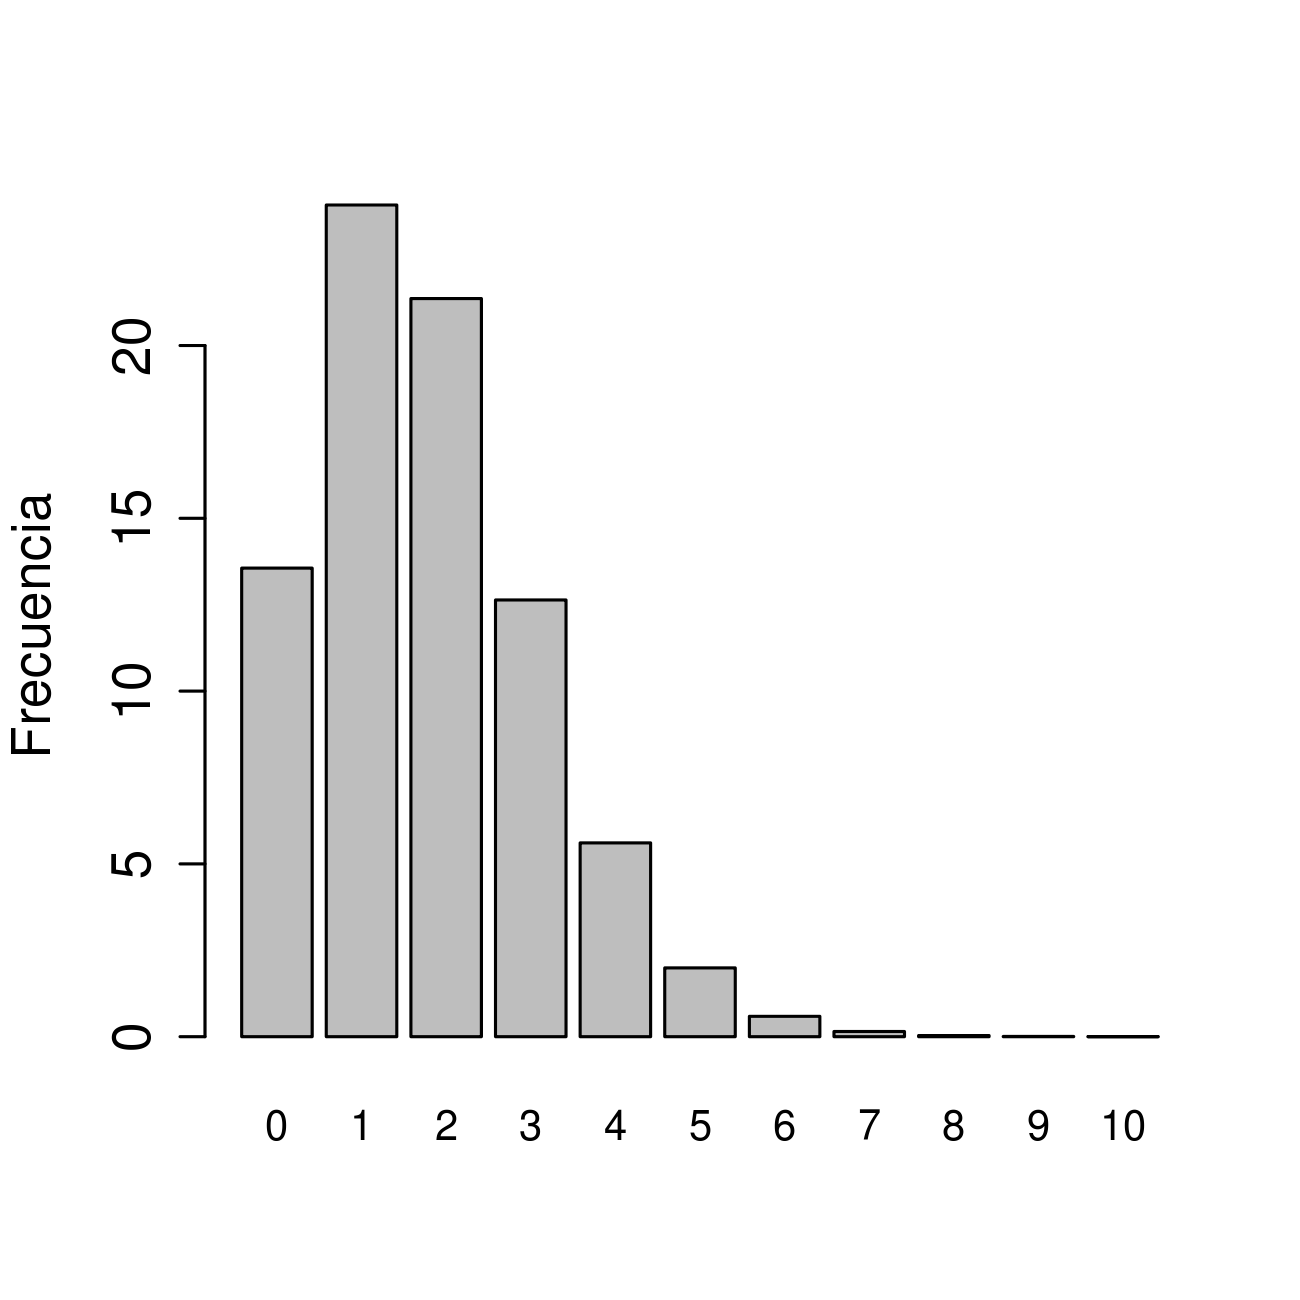
\includegraphics[scale=0.55]{figs/PoissDist.png}
         \end{figure}
\end{frame}%
\note[itemize]{
   \item  ejemplo: distribuci\'on de Poisson teorica si el n\'umero de bancos quebrados entre paises es completamente aleatorio
   \item Parece similar a la distribucion binomial no cierto? distribucion binomial con probabilidad baja y muestra grande, es equivalente a una distribucion de Poisson. 
              }%%}}}
%%}}}


% ===== SUBSECTION: Normal distribution =====%%%{{{
\subsection[Normal]{Distribuci\'on de Normal}

% ----- Normal distribution [label=normdist1] ----- %%{{{
\begin{frame}[label=normdist1]
   \frametitle{Distribuci\'on normal}
   \framesubtitle{Definici\'on}
   \begin{itemize}[<+-| handout:1>]
      \item Teorema del l\'imite central 
      \item Suficientes muestras $\rightarrow$ medias $\rightarrow$ distribuci\'on normal
   \end{itemize}
   \visible<3-| handout:1>{\begin{beamerboxesrounded}{}
   \begin{itemize}[<+-| handout:1>]
   \item Distribuci\'on continua
   \item $X \leadsto \mathcal{N}(\mu,\sigma)$
   \item $f(y)=\frac{1}{\sqrt{2\pi\sigma^2}}e^{-\frac{1}{2}\left( \frac{y-\mu}{\sigma}\right)^2}$
   \end{itemize}
   \end{beamerboxesrounded}
   }
\end{frame}%%%}}}


% ----- Normal distribution [label=normdist2] ----- %%{{{
\begin{frame}[label=normdist2]
   \frametitle{Distribuci\'on normal}
   \framesubtitle{¿Cuando se aplica?}

   \begin{itemize}
      \item ¡Todo el tiempo! 
      \item Regresi\'on lineal, an\'alisis de varianza \ldots 
   \end{itemize}
   \vspace{-1cm}
   \visible<2-| handout:1>{\begin{figure}
      \includegraphics<1| handout:0>[scale=0.6]{figs/NormDist1.png}
      \includegraphics<2| handout:0>[scale=0.6]{figs/NormDist2.png}
      \includegraphics<3| handout:0>[scale=0.6]{figs/NormDist3.png}
      \includegraphics<4| handout:0>[scale=0.6]{figs/NormDist4.png}
      \includegraphics<5| handout:1>[scale=0.6]{figs/NormDist5.png}
   \end{figure}
   }
\end{frame}%
\note[itemize]{
   \item no simetrico porque lo corte
}%%}}}


% ----- Standard Normal Distribution [label=stdnorm] ----- %%{{{
\begin{frame}[label=stdnorm]
   \frametitle{Distribuci\'on Normal Est\'andar}
   \framesubtitle{$X \leadsto \mathcal{N}(0,1)$}
   \vspace{-0.5cm}
   \begin{columns}[c, totalwidth=10cm]
      \begin{column}[]{6cm}
         \begin{figure}
            \includegraphics<1| handout:0>[scale=0.65]{figs/NormDist7.png}
            \includegraphics<2| handout:1>[scale=0.65]{figs/NormDist8.png}
            \includegraphics<3| handout:2>[scale=0.65]{figs/NormDist9.png}
            \includegraphics<4| handout:3>[scale=0.65]{figs/NormDist10.png}
         \end{figure}
      \end{column}
      \begin{column}[]{3.5cm}
         \begin{itemize}
            \item<2| handout:1> $\pm~1~\sigma \sim 68\%$
            \item<3| handout:2> $\pm~2~\sigma \sim 95\%$
            \item<4| handout:3> $\pm~3~\sigma \sim 99\%$
         \end{itemize}
      \end{column}
   \end{columns}
\end{frame}%%%}}}
%%}}}


% ===== SUBSECTION: Other distributions =====%%%{{{
\subsection[Otras]{Otras distribuci\'on}

% ----- Other distributions 1 [label=otherdist1] ----- %%{{{
\begin{frame}[label=otherdist1]
   \frametitle{Otras distribuciones de variables}
   \begin{itemize}
      \item Lognormal (largo, peso \ldots)
      \item Exponencial (Tiempo de fracaso)
      \item Gamma
      \item Distribuci\'on de Weibull
      \item Beta
   \end{itemize}
\end{frame}%%%}}}


% ----- Other distributions 2 [label=otherdist2] ----- %%{{{
\begin{frame}[label=otherdist2]
   \frametitle{Distribuciones de estad\'isticos}
   \begin{itemize}
      \item Distribuci\'on $z$ 
      \item Distribuci\'on $t$ de Student
      \item Distribuci\'on del $\chi^2$ 
      \item Distribuci\'on $F$ de Fischer
   \end{itemize}
\end{frame}%%%}}}
%%}}}




% ==================== SECTION: Test procedure ====================
\section[Procedimiento]{Procedimiento de los tests estad\'isticos}

% ===== SUBSECTION: Procedure =====%%%{{{
\subsection[?`Qu\'e es un test?]{?`Qu\'e es un test?}

% ----- What is a statistical test? [label=testdef] ----- %%{{{
\begin{frame}[label=testdef]
   \frametitle{?`Qu\'e es un test estad\'istico?}
   \framesubtitle{Herramienta para tomar decisi\'on}
   \begin{itemize}
      \item Calcular un estad\'istico $T_{obs}$ de una muestra
      \item Comparar $T_{obs}$ con la distribuci\'on de $T_{teo}$ cuando la hip\'otesis es verdadera
      \item La posici\'on de $T_{obs}$ informa sobre la probabilidad de que la hip\'otesis sea verdadera
   \end{itemize}
\end{frame}%%%}}}
%%}}}


% ===== SUBSECTION: overview =====%%%{{{
\subsection[Generalidades]{Visi\'on general}

% ----- Statistical test procedure [label=testproc1]----- %%{{{
\begin{frame}[label=testproc1]
   \frametitle{Test estad\'istico: procedimiento}
   \begin{enumerate}[<+-| handout:1>]
      \item Pregunta biol\'ogica: ¿Hay c\'ondores en el parque?
      \item Pregunta estad\'istica: Hip\'otesis $H_0$
      \item Elecci\'on del test estad\'istico: ¿Cu\'al usar?
      \item Criterios de decisi\'on: ¿Qu\'e riesgo de error? ¿Qu\'e nivel de confianza?
   \end{enumerate}
\end{frame}%%%}}}


% ----- Statistical test procedure [label=testproc2]----- %%{{{
\begin{frame}[label=testproc2]
   \frametitle{Test estad\'istico: procedimiento}
   \begin{enumerate}[<+-| handout:1>]
      \setcounter{enumi}{4}
      \item \alert<.| handout:1>{¡Colecci\'on de los datos!}
      \item C\'alculo de el estad\'istico del test
      \item Decisi\'on estad\'istica: ¿Se puede rechazar $H_0$ o no?
      \item Inferencia y explicaci\'on biol\'ogica
   \end{enumerate}
\end{frame}%%%}}}
%%}}}


% ===== SUBSECTION: Hypothese =====%%%{{{
\subsection[Hip\'otesis]{Hip\'otesis}

% ----- Good and bad hypoheses [label=popper] ----- %%{{{
\begin{frame}[label=popper]
\frametitle{Buenas y malas hip\'otesis}
\begin{itemize}
   \item Una buena hip\'otesis \alert<1| handout:1>{se puede rechazar/falsear} 
\end{itemize}
\begin{enumerate}[<+(1)-| visible@+(1)-| handout:1>]
   \item Hay c\'ondores en el parque
   \item No hay c\'ondores en el parque
\end{enumerate}
\begin{itemize}[<4-| visible@4-| handout:1>]
   \item \alert<.| handout:1>{¡Ausencia de prueba no es prueba de ausencia!}
\end{itemize}
\end{frame}%
\note[itemize]{
   \item como van a refutar esta hip\'otesis? 
   \item Van al parque y buscan los c\'ondores.  no ven ninguno. No significa que no hab\'ia condores. Quiz\'as les vieron venir y se escondieron. No importa cu\'anto tiempo van a mirar, nunca pueden refutar esta hip\'otesis. No pueden decir que la hip\'otesis es falsa. La \'unica cosa que pueden decir es ``fui al parque y no vi ning\'un c\'ondor''
   \item Ahora, este segunda hip\'otesis. La idea es la misma, no cierto?. Pero tan pronto como ven un c\'ondor, pueden rechazar la hip\'otesis. Hasta que realmente ven un c\'ondor, trabajan con la condici\'on de que la hip\'otesis es verdadera pero si ven un c\'ondor, la hip\'otesis es obviamente falsa y pueden rechazarla
              }%%}}}


% ----- Null hypothesis [label=null] ----- %%{{{
\begin{frame}[label=null]
\frametitle{Hip\'otesis nula}
 \begin{itemize}[<+-| handout:1>]
   \item ``Nada est\'a pasando''
   \item ``Las medias de dos muestras son las mismas'' 
   \item ``La pendiente de la relaci\'on es cero''
\end{itemize}
\medskip
\begin{itemize}[<+-| handout:1>]
\item[$\Rightarrow$] La hip\'otesis nula \alert{se puede falsear}. Rechazar cuando los datos muestran que es suficientemente improbable
\end{itemize}
\end{frame}%%%}}}
%%}}}


% ===== SUBSECTION: Test procedure =====%%%{{{
\subsection[Procedimiento]{Procedimiento}

% ----- Test choice overview [label=testchoice] ----- %%{{{
\begin{frame}[label=testchoice]
   \frametitle{Elecci\'on del test}
   \begin{itemize}
      \item Tipo de variables: cualitativas, cuantitativas \ldots
      \item N\'umero y tama\~no de las muestras
      \item Condiciones de cada test
   \end{itemize}
\end{frame}%%%}}}
%%}}}


% ===== SUBSECTION: Decision criterions =====%%%{{{
\subsection[Decisi\'on]{Criterios de decisi\'on}

% ----- Decision criterions 1 [label=critdecis1] ----- %%{{{
\begin{frame}[label=critdecis1]
   \frametitle{Criterios de decisi\'on (1)}
   \begin{columns}[c, totalwidth=10cm]
      \begin{column}[]{5.5cm}
         \begin{figure}
            \includegraphics<1| handout:0>[scale=0.6]{figs/NormDist9.png}
            \includegraphics<2-3| handout:1>[scale=0.6]{figs/PrincipTest1.png}
            \includegraphics<4-| handout:2>[scale=0.6]{figs/PrincipTest2.png}
         \end{figure}
      \end{column}
      \begin{column}[]{4.5cm}
         \begin{itemize}
            \item<1-3| handout:1> $\pm~2~\sigma \sim 95\%$
            \item<2-3| handout:1> Valores umbrales
            \item<3| handout:1> Regi\'on de aceptaci\'on
            \item<4-| handout:2> $5\%$ menos probable 
            \item<5-| handout:2> Regi\'on de rechazo
            \item<6-| handout:2> \alert{Riesgo $\alpha$}
         \end{itemize}
      \end{column}
   \end{columns}
\end{frame}%%%}}}


% ----- Decision criterions 2 [label=critdecis2] ----- %%{{{
\begin{frame}[label=critdecis2]
   \frametitle{Criterios de decisi\'on (2)}
   \begin{itemize}
      \item 2 errores posibles :
      \begin{description}[Tipo II]
         \item[Tipo I]: Rechazar $H_0$ cuando es verdadera
         \item[Tipo II]: Aceptar $H_0$ cuando es falsa
      \end{description}
   \end{itemize}
   \smallskip
   \footnotesize
   \renewcommand{\arraystretch}{1.8}
   \renewcommand{\tabcolsep}{0.2cm}
   \pause
   \begin{table}
      \begin{tabular}{ccc}
         \firsthline
            & \multicolumn{2}{c}{ Situaci\'on real} \\
         \cline{2-3} Hip\'otesis nula & \uncover<2,4| handout:1>{Verdadera}
         & \uncover<3,5| handout:1>{Falsa} \\ \hline \uncover<2,5>{Acepta}
         & \uncover<2| handout:1>{\begin{minipage}[c]{20ex}
                          \begin{center}
                             \vspace{3pt}
                             \alert<2| handout:1>{Decisi\'on correcta \\ Poder $1-\beta$ }
                             \vspace{3pt}
                          \end{center}
                       \end{minipage}  
                           } &
         \uncover<5| handout:1>{\begin{minipage}[c]{20ex}
                        \begin{center}
                           \vspace{3pt}
                           \alert<5| handout:1>{Tipo II\\ Riesgo $\beta$}
                        \end{center}
                     \end{minipage}} \\ \uncover<3,4| handout:1>{Rechaza} &
         \uncover<4| handout:1>{\begin{minipage}[c]{20ex}
                        \begin{center}
                           \alert<4| handout:1>{Tipo I\\ Riesgo $\alpha$}
                           \vspace{3pt}
                        \end{center}
                     \end{minipage}
                     } & \uncover<3| handout:1>{\alert<3>{Decisi\'on correcta}} \\ 
                     \lasthline
      \end{tabular}
   \end{table}
\end{frame}%%%}}}
%%}}}


% ===== SUBSECTION: Power =====%%%{{{
\subsection[Poder]{Poder de un test}

% ----- Power 1 [label=power1]----- %%{{{
\begin{frame}[label=power1]
   \frametitle{Hay que comprometer \ldots}
   \begin{beamerboxesrounded}{}
      Poder: Probabilidad de rechazar $H_0$ cuando es falsa
   \end{beamerboxesrounded}
   \onslide<2-| handout:1>{\begin{itemize}
      \item<3-| handout:1> Error I: rechazar $H_0$ cuando es verdadera \alert<.>{$\alpha$}
      \item<4-| handout:1> Error II: aceptar $H_0$ cuando es falsa \alert<.>{$\beta$}
      \item<5-| handout:1> Poder: $1-\beta$
      \item<6-| handout:1> $\alpha$ y $\beta$ relacionados
      \item<7-| handout:1> Cuando $\alpha$ $\searrow$ $\beta$ $\nearrow$
   \end{itemize}
   }
\end{frame}%%%}}}


% ----- Beta high 2 [label=betahigh1] ----- %%{{{
\begin{frame}[label=betahigh1]
   \frametitle{?`Cuando $\alpha$ \emph{debe} ser alto?}
   \begin{exampleblock}{Ejemplo: Efectos secundarios de una droga}
      \begin{itemize}
         \item Test final antes de comercializar
         \item Grupo A: droga $|$ Grupo B: placebo
         \item $H_0$: no hay diferencia entre grupos A y B
         \item $H_1$: A tiene mayor frecuencia de anomal\'ias que B
      \end{itemize}
   \end{exampleblock}
\end{frame}%%%}}}


% ----- Beta high 2 [label=betahigh2] ----- %%{{{
\begin{frame}[label=betahigh2]
   \frametitle{?`Cu\'ando $\alpha$ \emph{debe} ser alto?}
   \framesubtitle{Aceptar riesgo $\alpha$ m\'as alto para reducir riesgo $\beta$  }
   \begin{block}{$\alpha$ alto: error de tipo I}
      \begin{itemize}
         \item $H_0$ rechazada pero verdadera 
         \item No se comercializa
         \item M\'as estudios para determinar efecto real
      \end{itemize}
   \end{block}

   \visible<2-| handout:1>{\begin{alertblock}{$\beta$ alto: error de tipo II}
      \begin{itemize}
         \item $H_0$ ``aceptada'' pero falsa
         \item Comercializaci\'on 
         \item !`Mucha gente sufre de los efectos secundarios!
      \end{itemize}
   \end{alertblock}
               }
\end{frame}%%%}}}
%%}}}


% ===== SUBSECTION: Data collection =====%%%{{{
\subsection[Colleci\'on de datos]{Colleci\'on de datos}

% ----- Data collection [label=datacoll] ----- %%{{{
\begin{frame}[label=datacoll]
   \frametitle{Colecci\'on de los datos}
   \begin{beamerboxesrounded}{¡Acu\'erdense!}
      \begin{itemize}
         \item Aleatorizaci\'on
         \item Replicaci\'on
      \end{itemize}
   \end{beamerboxesrounded}
\end{frame}%%%}}}
%%}}}


% ===== SUBSECTION: Test computation =====%%%{{{
\subsection[C\'alculo]{C\'alculo del test}

% ----- Computation of test statistic [label=teststat] ----- %%{{{
\begin{frame}[label=teststat]
   \frametitle{Computaci\'on del estad\'istico del test}
   \begin{exampleblock}{Ejemplo: Prevalencia de la malaria}
   \vspace{2ex}
   \begin{itemize}[<+-| handout:1>]
      \item ``La prevalencia es la misma en A y en B''
      \item $H_0: \mu_A = \mu_B$
      \item El estad\'istico del test representa la diferencia de prevalencia: $T=f(prev_A - prev_B)$ 
      \item Distribuci\'on de $T$ corresponde a $H_0$ verdadera
   \end{itemize}
   \end{exampleblock}
\end{frame}%%%}}}


% ----- Positioning of test statistic 1 [label=testpos1] ----- %%{{{
\begin{frame}[label=testpos1]
   \frametitle{Comparaci\'on de $T$ con la distribuci\'on te\'orica}
   \vspace{-0.5cm}
   \begin{columns}[c,totalwidth=10cm]
      \begin{column}[]{4.5cm}
         \begin{figure}
            \includegraphics<1| handout:1>[scale=0.55]{figs/testpos1.png}
         \end{figure}
      \end{column}
      \begin{column}[]{4.5cm}
         \begin{itemize}
            \item $T_{obs}$ no est\'a en la regi\'on de rechazo
            \item No se puede rechazar $H_0$
            \item No es posible afirmar que hay una diferencia de prevalencia entre A y B
            \item[] 
         \end{itemize}
      \end{column}
   \end{columns}
\end{frame}%%%}}}


% ----- Positioning of test statistic 2 [label=testpos2] ----- %%{{{
\begin{frame}[label=testpos2]
   \frametitle{Comparaci\'on de $T$ con la distribuci\'on te\'orica}
   \vspace{-0.5cm}
   \begin{columns}[c,totalwidth=10cm]
      \begin{column}[]{4.5cm}
         \begin{figure}
            \includegraphics<1| handout:1>[scale=0.55]{figs/testpos2.png}
         \end{figure}
      \end{column}
      \begin{column}[]{4.5cm}
         \begin{itemize}
            \item $T_{obs}$ est\'a en la regi\'on de rechazo
            \item Se puede rechazar $H_0$
            \item Se concluye que la prevalencia de la malaria es diferente entre A y B
            \item El riesgo de que esta conclusi\'on sea falsa es $\alpha=5\%$
         \end{itemize}
      \end{column}
   \end{columns}
\end{frame}%%%}}}
%%}}}


% ===== SUBSECTION: P-Value =====%%%{{{
\subsection[Valor $P$]{Valor $P$}

%% ----- P-value [label=pvalue1] ----- %%{{{
\begin{frame}[label=pvalue1]
\frametitle{Valor $P$}

\begin{itemize}
   \item Medida de la credibilidad de la hip\'otesis nula
\end{itemize}

\visible<2-| handout:1>{
   \begin{exampleblock}{Ejemplo}
      \begin{itemize}
         \item<2-| uncover@2-| handout:1> $H_0: \mu_A = \mu_B$
         \item \onslide<3-| handout:1>{$p < 0.05$ \visible<4>{\alert<4>{$\Rightarrow$ improbable que $H_0$ sea verdadera: $\mu_A \neq \mu_B$}}%
         }
         \item \onslide<5-| handout:1>{$p=0.23$ \visible<6>{\alert<6>{$\Rightarrow$ No hay suficiente evidencia para rechazar $H_0$ }}%
                           }
      \end{itemize}
   \end{exampleblock}
}
\end{frame}
\note[itemize]{
   \item Probabilidad de que un resultado m\'as extremo que lo que fue observado podria haber occurrrido por azar, si la hip\'otesis nula ser\'ia verdadera
\item valor p is the surface below the curve: the fraction of the sampling distribution that is at least as extreme as the observed value 
}%%}}}
%%}}}


% ===== SUBSECTION: SIGNIFICANCE  =====%%%{{{
\subsection[Significancia]{Significancia}

% ----- Significance [label=signif1] ----- %%{{{
\begin{frame}[label=signif1]
\frametitle{Significancia}
 \begin{itemize}[<+- | uncover+| handout:1>]
   \item ¿Qu\'e significa ``Resultado significativo''?
   \item Diccionario: Que tiene sentido
   \item Estad\'istica: Improbable que haya ocurrido por azar \onslide<4-| handout:1>{si la hip\'otesis nula es verdadera}
   \item<5-| handout:1> Improbable: Occurre menos de $5\%$ de las veces
\end{itemize}
\end{frame}%%%}}}
%%}}}




% ==================== SECTION: Test choice ====================
\section[?`Cu\'al test?]{Elegir el test adecuado}

% ===== SUBSECTION: Decision tree =====%%%{{{
\subsection[Arb\'ol de decisi\'on]{Arb\'ol de decisi\'on}

% ----- Choice of test 1 [label=chtest1] -----%%{{{
\begin{frame}[label=chtest1]
   \frametitle{?`Como elegir el test adecuado?}
   \framesubtitle{Algunas directrices (1)}
   \scriptsize
   
%% tikz code for figure choicetest1
%% used on line 1606 of main.text

\begin{tikzpicture}
\node {Tipo de variable} [grow'=right, ->]
   child {node {Cualitativa}
         }
   child[missing] {node {}}
   child {node {Cuantitativa}
            child [level distance=2cm] {node {$\mathcal{N}(\mu,\sigma)$}
                     {child [level distance=2cm] {node {\parbox[c]{12ex}{\centering Test param\'etrico}}}}
                  }
            child[missing] {node {}}
            child [level distance=2cm] {node {\parbox[c]{12ex}{\centering No distribuci\'on }}
                     {child [level distance=2cm] {node {\parbox[c]{12ex}{\centering Test no param\'etrico}}}}
                  }
         } ;

\end{tikzpicture}

\end{frame}%%%}}}


% ----- Choice of test 2 [label=chtest2] ----- %%{{{
\begin{frame}[label=chtest2]
   \frametitle{?`Como elegir el test adecuado?}
   \framesubtitle{Algunas directrices (2)}
   \scriptsize
   %%% tikz code for figure choicetest2
%% used on line 1615 of main.tex
\begin{tikzpicture}
\node {\parbox[c]{11ex}{N\'umero de muestras}} [grow'=right, ->]
      child {node {1}}
      child {node {2}
        child {node {Asociadas}} 
        child {node {No}}
            }
      child[missing] {node {}}
      child {node {$k$}
        child {node {Asociadas}} 
        child {node {No}}
            } ;
\end{tikzpicture}

   \normalsize
\end{frame}%%}}}


% ----- Dependence Pairing [label=deppair] ----- %%{{{
\begin{frame}[label=deppair]
   \frametitle{Dependencia -- Asociaci\'on}
   \framesubtitle{Tests asociados}
   \begin{itemize}
      \item Muestras asociadas: vienen del mismo grupo
      \item Relacionadas por correlaci\'on o por regresi\'on
      \item Conexi\'on espacial
      \item Conexi\'on temporal
      \vspace{1ex}
      \item[$\Rightarrow$] Usar tests espec\'ificos: e.g., ``paired t-test''
   \end{itemize}
\end{frame}%%%}}}
%%}}}


% ===== SUBSECTION: Comparison tests =====%%%{{{
\subsection[Comparaci\'on]{Tests de comparaci\'on}

% ----- Choice of test 3 [label=chtest3] ----- %%{{{
\begin{frame}[label=chtest3]
   \frametitle{Comparar una muestra con una distribuci\'on te\'orica }
   \begin{block}{\alert{$\Rightarrow$ Test de conformidad}}
   \begin{itemize}
      \item Test $t$ de conformidad
      \item Test de Wilcoxon
      \item Test binomial
      \item Test $\chi^2$ de conformidad
      \item \ldots
   \end{itemize}
   \end{block}
\end{frame}%%%}}}

 
% ----- Choice of test 4 [label=chtest4] ----- %%{{{
\begin{frame}[label=chtest4]
   \frametitle{Comparar dos muestras}
   \begin{block}{\alert{$\Rightarrow$ Test de comparaci\'on (de homogeneidad)}}
   \begin{itemize}
      \item Test $t$ (posiblemente ``asociado'')
      \item Test de Mann-Whitney
      \item Test de Fisher
      \item Test $\chi^2$
      \item \ldots
   \end{itemize}
   \end{block}
\end{frame}%%%}}}


% ----- Choice of test 5 [label=chtest5] ----- %%{{{
\begin{frame}[label=chtest5]
   \frametitle{Comparar \emph{m\'as} de dos muestras}
   \begin{block}{\alert{$\Rightarrow$ Test de comparaci\'on (continuaci\'on)}}
      \begin{itemize}
         \item Anova / Manova
         \item Test de Kruskal-Wallis
         \item Test de Friedman
         \item Test $\chi^2$
         \item \ldots
      \end{itemize}
   \end{block}
  \end{frame}%%%}}}
%%}}}


% ===== SUBSECTION: Association tests =====%%%{{{
\subsection[Asociaci\'on]{Tests de asociaci\'on}
 
% ----- Choice of test 6 [label=chtest6] ----- %%{{{
\begin{frame}[label=chtest6]
   \frametitle{Evaluar el grado de asociaci\'on entre variables}
   \framesubtitle{Muestras independientes}
   \begin{block}{\alert{$\Rightarrow$ Correlaci\'on y regresi\'on}}
      \begin{itemize}
         \item Correlaci\'on de Pearson / de Spearman ($n=2$)
         \item Regresi\'on simple / regresi\'on log\'istica (n=2)
         \item Regresi\'on no param\'etrica
         \item Regresi\'on m\'ultiple / regresi\'on log\'istica m\'ultiple ($n>2$)
         \item \ldots
      \end{itemize}
   \end{block}
\end{frame}%%%}}}
%%}}}

  
% ===== SUBSECTION: More directions =====%%%{{{
\subsection[M\'as directrices]{M\'as directrices para elegir un test}

% ----- Choice of test 7 [label=chtest7] ----- %%{{{
\begin{frame}[label=chtest7,plain]
   \vspace{-1cm}
   \begin{overprint}
      \only<1| handout:1>{\frametitle{Comparar un grupo con una distribuci\'on te\'orica} }
      \only<2| handout:2>{\frametitle{Comparar $2$ grupos no asociados\hspace{10ex} } }
      \only<3| handout:3>{\frametitle{Comparar $2$ grupos asociados\hspace{10ex} } }
      \only<4| handout:4>{\frametitle{Comparar $\geq3$ grupos no asociados\hspace{10ex}} }
      \only<5| handout:5>{\frametitle{Comparar $\geq3$ grupos asociados\hspace{10ex} } }
      \only<6| handout:6>{\frametitle{Cuantificar asociaci\'on entre 2 variables}}
      \only<7| handout:7>{\frametitle{Predecir valor desde $1$ variable\hspace{10ex} } }
      \only<8| handout:8>{\frametitle{Predecir valor desde varias variables}}
   \end{overprint}

   \renewcommand{\arraystretch}{1.5}
  \scriptsize
   % tikz code for table named tablechoice
%% on line 1724 of main.tex

\newcolumntype{V}[1]{%
  >{\scriptsize\raggedright\hspace{0pt}}m{#1}%
}

\newcolumntype{T}[1]{%
  >{\begin{center}\vspace{-1.5ex}}m{#1}<{\vspace{-1.5ex}\end{center}}%
}


\begin{overlayarea}{\textwidth}{5cm}

      \only<1| handout:1>{
      \begin{tabular}[c]{lll}
         \firsthline 
         \multicolumn{1}{T{2.2cm}@{}}{\structure{Medidas\\ $X\leadsto\mathcal{N}(\mu,\sigma)$}} &  \multicolumn{1}{T{2.2cm}@{}}{\structure{Categor\'ia, grado, \\ sin distribuci\'on}} & \multicolumn{1}{T{2.2cm}@{}}{\structure{Binomial}} \\
         \hline 
         \multicolumn{1}{V{3cm}@{}}{Test $t$ 1 muestra} & \multicolumn{1}{V{3cm}@{}}{Test de Wilcoxon} & \multicolumn{1}{V{3cm}@{}}{Test $\chi^2$, test binomial}  \\
         \lasthline
     \end{tabular} 
              }%

   \only<2| handout:2>{%
      \begin{tabular}[c]{lll}
         \firsthline 
         \multicolumn{1}{T{2.2cm}@{}}{\structure{Medidas\\ $X\leadsto\mathcal{N}(\mu,\sigma)$}} &  \multicolumn{1}{T{2.2cm}@{}}{\structure{Categor\'ia, grado, \\ sin distribuci\'on}} & \multicolumn{1}{T{2.2cm}@{}}{\structure{Binomial}} \\
         \hline 
         \multicolumn{1}{V{3cm}@{}}{Test $t$ 1 muestra} & \multicolumn{1}{V{3cm}@{}}{Test de Wilcoxon} & \multicolumn{1}{V{3cm}@{}}{Test $\chi^2$, test binomial}  \\
         \multicolumn{1}{V{3cm}@{}}{Test $t$ no asociado} & \multicolumn{1}{V{3cm}@{}}{Test de Mann-Whitney} & \multicolumn{1}{V{3cm}@{}}{Test de Fisher, test $\chi^2$}  \\
         \lasthline
      \end{tabular}
           }%

\only<3| handout:3>{%
      \begin{tabular}[c]{lll}
         \firsthline 
         \multicolumn{1}{T{2.2cm}@{}}{\structure{Medidas\\ $X\leadsto\mathcal{N}(\mu,\sigma)$}} &  \multicolumn{1}{T{2.2cm}@{}}{\structure{Categor\'ia, grado, \\ sin distribuci\'on}} & \multicolumn{1}{T{2.2cm}@{}}{\structure{Binomial}} \\
         \hline 
         \multicolumn{1}{V{3cm}@{}}{Test $t$ 1 muestra} & \multicolumn{1}{V{3cm}@{}}{Test de Wilcoxon} & \multicolumn{1}{V{3cm}@{}}{Test $\chi^2$, test binomial}  \\
         \multicolumn{1}{V{3cm}@{}}{Test $t$ no asociado} & \multicolumn{1}{V{3cm}@{}}{Test de Mann-Whitney} & \multicolumn{1}{V{3cm}@{}}{Test de Fisher, test $\chi^2$}  \\
         \multicolumn{1}{V{3cm}@{}}{Test $t$ asociado} & \multicolumn{1}{V{3cm}@{}}{Test de Wilcoxon} & \multicolumn{1}{V{3cm}@{}}{Test de McNemar}  \\
         \lasthline
      \end{tabular}
           }%

\only<4| handout:4>{%
      \begin{tabular}[c]{lll}
         \firsthline 
         \multicolumn{1}{T{2.2cm}@{}}{\structure{Medidas\\ $X\leadsto\mathcal{N}(\mu,\sigma)$}} &  \multicolumn{1}{T{2.2cm}@{}}{\structure{Categor\'ia, grado, \\ sin distribuci\'on}} & \multicolumn{1}{T{2.2cm}@{}}{\structure{Binomial}} \\
         \hline 
         \multicolumn{1}{V{3cm}@{}}{Test $t$ 1 muestra} & \multicolumn{1}{V{3cm}@{}}{Test de Wilcoxon} & \multicolumn{1}{V{3cm}@{}}{Test $\chi^2$, test binomial}  \\
         \multicolumn{1}{V{3cm}@{}}{Test $t$ no asociado} & \multicolumn{1}{V{3cm}@{}}{Test de Mann-Whitney} & \multicolumn{1}{V{3cm}@{}}{Test de Fisher, test $\chi^2$}  \\
         \multicolumn{1}{V{3cm}@{}}{Test $t$ asociado} & \multicolumn{1}{V{3cm}@{}}{Test de Wilcoxon} & \multicolumn{1}{V{3cm}@{}}{Test de McNemar}  \\
         \multicolumn{1}{V{3cm}@{}}{Anova simple} & \multicolumn{1}{V{3cm}@{}}{Test de Kruskal-Wallis} & \multicolumn{1}{V{3cm}@{}}{Test $\chi^2$}  \\
         \lasthline
      \end{tabular}
           }%

\only<5| handout:5>{%
      \begin{tabular}[c]{lll}
         \firsthline 
         \multicolumn{1}{T{2.2cm}@{}}{\structure{Medidas\\ $X\leadsto\mathcal{N}(\mu,\sigma)$}} &  \multicolumn{1}{T{2.2cm}@{}}{\structure{Categor\'ia, grado, \\ sin distribuci\'on}} & \multicolumn{1}{T{2.2cm}@{}}{\structure{Binomial}} \\
         \hline 
         \multicolumn{1}{V{3cm}@{}}{Test $t$ 1 muestra} & \multicolumn{1}{V{3cm}@{}}{Test de Wilcoxon} & \multicolumn{1}{V{3cm}@{}}{Test $\chi^2$, test binomial}  \\
         \multicolumn{1}{V{3cm}@{}}{Test $t$ no asociado} & \multicolumn{1}{V{3cm}@{}}{Test de Mann-Whitney} & \multicolumn{1}{V{3cm}@{}}{Test de Fisher, test $\chi^2$}  \\
         \multicolumn{1}{V{3cm}@{}}{Test $t$ asociado} & \multicolumn{1}{V{3cm}@{}}{Test de Wilcoxon} & \multicolumn{1}{V{3cm}@{}}{Test de McNemar}  \\
         \multicolumn{1}{V{3cm}@{}}{Anova simple} & \multicolumn{1}{V{3cm}@{}}{Test de Kruskal-Wallis} & \multicolumn{1}{V{3cm}@{}}{Test $\chi^2$}  \\
         \multicolumn{1}{V{3cm}@{}}{Anova con medidas repetidas} & \multicolumn{1}{V{3cm}@{}}{Test de Friedman} & \multicolumn{1}{V{3cm}@{}}{Test $
         Q$ de Cochran}  \\
         \lasthline
      \end{tabular}
           }%

\only<6| handout:6>{%
      \begin{tabular}[c]{lll}
         \firsthline 
         \multicolumn{1}{T{2.2cm}@{}}{\structure{Medidas\\ $X\leadsto\mathcal{N}(\mu,\sigma)$}} &  \multicolumn{1}{T{2.2cm}@{}}{\structure{Categor\'ia, grado, \\ sin distribuci\'on}} & \multicolumn{1}{T{2.2cm}@{}}{\structure{Binomial}} \\
         \hline 
         \multicolumn{1}{V{3cm}@{}}{Test $t$ 1 muestra} & \multicolumn{1}{V{3cm}@{}}{Test de Wilcoxon} & \multicolumn{1}{V{3cm}@{}}{Test $\chi^2$, test binomial}  \\
         \multicolumn{1}{V{3cm}@{}}{Test $t$ no asociado} & \multicolumn{1}{V{3cm}@{}}{Test de Mann-Whitney} & \multicolumn{1}{V{3cm}@{}}{Test de Fisher, test $\chi^2$}  \\
         \multicolumn{1}{V{3cm}@{}}{Test $t$ asociado} & \multicolumn{1}{V{3cm}@{}}{Test de Wilcoxon} & \multicolumn{1}{V{3cm}@{}}{Test de McNemar}  \\
         \multicolumn{1}{V{3cm}@{}}{Anova simple} & \multicolumn{1}{V{3cm}@{}}{Test de Kruskal-Wallis} & \multicolumn{1}{V{3cm}@{}}{Test $\chi^2$}  \\
         \multicolumn{1}{V{3cm}@{}}{Anova con medidas repetidas} & \multicolumn{1}{V{3cm}@{}}{Test de Friedman} & \multicolumn{1}{V{3cm}@{}}{Test $Q$ de Cochran}  \\
         \multicolumn{1}{V{3cm}@{}}{Correlaci\'on de Pearson} & \multicolumn{1}{V{3cm}@{}}{Correlaci\'on de Spearman} & \multicolumn{1}{V{3cm}@{}}{Coeficientes de contingencia}  \\
         \lasthline
      \end{tabular}
           }%

\only<7| handout:7>{%
      \begin{tabular}[c]{lll}
         \firsthline 
         \multicolumn{1}{T{2.2cm}@{}}{\structure{Medidas\\ $X\leadsto\mathcal{N}(\mu,\sigma)$}} &  \multicolumn{1}{T{2.2cm}@{}}{\structure{Categor\'ia, grado, \\ sin distribuci\'on}} & \multicolumn{1}{T{2.2cm}@{}}{\structure{Binomial}} \\
         \hline 
         \multicolumn{1}{V{3cm}@{}}{Test $t$ 1 muestra} & \multicolumn{1}{V{3cm}@{}}{Test de Wilcoxon} & \multicolumn{1}{V{3cm}@{}}{Test $\chi^2$, test binomial}  \\
         \multicolumn{1}{V{3cm}@{}}{Test $t$ no asociado} & \multicolumn{1}{V{3cm}@{}}{Test de Mann-Whitney} & \multicolumn{1}{V{3cm}@{}}{Test de Fisher, test $\chi^2$}  \\
         \multicolumn{1}{V{3cm}@{}}{Test $t$ asociado} & \multicolumn{1}{V{3cm}@{}}{Test de Wilcoxon} & \multicolumn{1}{V{3cm}@{}}{Test de McNemar}  \\
         \multicolumn{1}{V{3cm}@{}}{Anova simple} & \multicolumn{1}{V{3cm}@{}}{Test de Kruskal-Wallis} & \multicolumn{1}{V{3cm}@{}}{Test $\chi^2$}  \\
         \multicolumn{1}{V{3cm}@{}}{Anova con medidas repetidas} & \multicolumn{1}{V{3cm}@{}}{Test de Friedman} & \multicolumn{1}{V{3cm}@{}}{Test $Q$ de Cochran}  \\
         \multicolumn{1}{V{3cm}@{}}{Correlaci\'on de Pearson} & \multicolumn{1}{V{3cm}@{}}{Correlaci\'on de Spearman} & \multicolumn{1}{V{3cm}@{}}{Coeficientes de contingencia}  \\
         \multicolumn{1}{V{3cm}@{}}{Regresi\'on (no)lineal simple} & \multicolumn{1}{V{3cm}@{}}{Regresi\'on no param\'etrica} & \multicolumn{1}{V{3cm}@{}}{Regresi\'on log\'istica simple}  \\
         \lasthline
      \end{tabular}
           }%

\only<8| handout:8>{%
      \begin{tabular}[c]{lll}
         \firsthline 
         \multicolumn{1}{T{2.2cm}@{}}{\structure{Medidas\\ $X\leadsto\mathcal{N}(\mu,\sigma)$}} &  \multicolumn{1}{T{2.2cm}@{}}{\structure{Categor\'ia, grado, \\ sin distribuci\'on}} & \multicolumn{1}{T{2.2cm}@{}}{\structure{Binomial}} \\
         \hline 
         \multicolumn{1}{V{3cm}@{}}{Test $t$ 1 muestra} & \multicolumn{1}{V{3cm}@{}}{Test de Wilcoxon} & \multicolumn{1}{V{3cm}@{}}{Test $\chi^2$, test binomial}  \\
         \multicolumn{1}{V{3cm}@{}}{Test $t$ no asociado} & \multicolumn{1}{V{3cm}@{}}{Test de Mann-Whitney} & \multicolumn{1}{V{3cm}@{}}{Test de Fisher, test $\chi^2$}  \\
         \multicolumn{1}{V{3cm}@{}}{Test $t$ asociado} & \multicolumn{1}{V{3cm}@{}}{Test de Wilcoxon} & \multicolumn{1}{V{3cm}@{}}{Test de McNemar}  \\
         \multicolumn{1}{V{3cm}@{}}{Anova simple} & \multicolumn{1}{V{3cm}@{}}{Test de Kruskal-Wallis} & \multicolumn{1}{V{3cm}@{}}{Test $\chi^2$}  \\
         \multicolumn{1}{V{3cm}@{}}{Anova con medidas repetidas} & \multicolumn{1}{V{3cm}@{}}{Test de Friedman} & \multicolumn{1}{V{3cm}@{}}{Test $Q$ de Cochran}  \\
         \multicolumn{1}{V{3cm}@{}}{Correlaci\'on de Pearson} & \multicolumn{1}{V{3cm}@{}}{Correlaci\'on de Spearman} & \multicolumn{1}{V{3cm}@{}}{Coeficientes de contingencia}  \\
         \multicolumn{1}{V{3cm}@{}}{Regresi\'on (no)lineal simple} & \multicolumn{1}{V{3cm}@{}}{Regresi\'on no param\'etrica} & \multicolumn{1}{V{3cm}@{}}{Regresi\'on log\'istica simple}  \\
         \multicolumn{1}{V{3cm}@{}}{Regresi\'on (no)lineal multiple} & \multicolumn{1}{V{3cm}@{}}{\rule[0ex]{1.5cm}{0.3pt}} & \multicolumn{1}{V{3cm}@{}}{Regresi\'on log\'istica multiple}  \\
         \lasthline
      \end{tabular}
           }%





\end{overlayarea}





\end{frame}%%%}}}


% ----- More help [label=chtest8] ----- %%{{{
\begin{frame}[label=chtest8]
   \frametitle{M\'as recursos para elegir un test}
   \hspace{-5cm}
   \small
    \begin{itemize}
      \item \emph{Handbook of Biological Statistics:} \\ \url{http://udel.edu/~mcdonald/statbigchart.html}
      \item \emph{Statistics Online Computational Resources:} \\ \url{www.socr.ucla.edu/Applets.dir/ChoiceOfTest.html}
      \item \emph{GraphPad / Intuitive Biostatistics:} \\ \url{www.graphpad.com/www/Book/Choose.htm}
      \item \emph{Social Research Methods:} \\ \url{www.socialresearchmethods.net/selstat/ssstart.htm}
      \item \emph{James D. Leeper, University of Alabama:} \\ \url{http://bama.ua.edu/~jleeper/627/choosestat.html}
      \item \emph{S. Holttum, B. Blizard, Canterbury Christ Church University:} \\ \url{www.whichtest.info/index.html}
   \end{itemize}
\end{frame}%%%}}}
%%}}}






% ==================== lecture - part 3 [label=titlepart3]====================
\lecture{Correlaci\'on y regresi\'on}{day3}
\part[Correlaci\'on y regresi\'on]{Correlaci\'on y regresi\'on}



% ================ SECTION Correlation Regression: Overview ===================
\section{Introduci\'on}
 

% ----- Context [label=regrcontext]----- %%{{{
\begin{frame}[label=regrcontext]
   \frametitle{Dos categor\'ias de tests estad\'isticos}
   \begin{description}
      \item[Tests de comparaci\'on]: $1$ variable, $\geq 2$ poblaciones
      \item[Tests de relaci\'on]: $\geq 2$ variables, $1$ poblaci\'on
   \end{description}
\end{frame}%%%}}}

 
% ----- Precisions [label=regrprec] ----- %%{{{
\begin{frame}[label=regrprec]
   \frametitle{$\geq 2$ variables es com\'un en biolog\'ia}
   \begin{exampleblock}{2 variables para el mismo individuo}
      \begin{itemize}
         \item Presi\'on sangu\'inea $X_1$, peso $X_2$
         \item Abundancia de una especie de planta $X_1$, nivel del pH en el suelo $X_2$, temperatura $X_3$ 
      \end{itemize}
   \end{exampleblock}
   \begin{itemize}
      \item Datos \alert{bi}variados o \alert{multi}variados
      \medskip
      \item[$\Rightarrow$] ?`Cu\'al es la relaci\'on entre las variables?
      %\item Descripci\'on de la relaci\'on entre variables
      %\item Uso de esta relaci\'on para hacer predicciones
   \end{itemize}
\end{frame}%%}}}


% ----- Overview 1 [label=corroverv1] ----- %%{{{
\begin{frame}[label=corroverv1]
   \frametitle{Relaci\'on entre $\geq 2$ variables}
   \framesubtitle{La estad\'istica correlacional}
   \begin{block}{Varios tipos de relaci\'on}
      \begin{itemize}
         \item No conexi\'on
         \item Relaci\'on $| handout:1>0$ / $<0$, causal / no
         \item Conexi\'on funcional $\rightarrow$ predicci\'on
      \end{itemize}
   \end{block}
   \begin{block}{Objetivo de la estad\'istica correlacional}
      \begin{itemize}
         \item Determinar validez y fuerza de la relaci\'on entre las variables
         \item Determinar la direcci\'on de la relaci\'on
      \end{itemize}
   \end{block}
\end{frame}%%}}}


% ----- Overview 2 [label=corroverv2] ----- %%{{{
\begin{frame}[label=corroverv2]
   \frametitle{Estad\'istica correlacional}
   \begin{description}[---------------------------]
       \item[Correlaci\'on:] ?`C\'omo 2 variables var\'ian juntas?
       \item[Regresi\'on:] Relaci\'on entre $1$ variable dependiente y $\geq 1$ variable independiente
       \item[An\'alisis multivariados:] Relaci\'on entre $\geq 2$ variables independientes / dependientes / ambos 
   \end{description}
\end{frame}%%%}}}



% ====================== SECTION Correlation ======================%
\section{Correlacii\'on}
 
% ===== SUBSECTION: Notion of correlation =====%%{{{
\subsection[Noci\'on de correlaci\'on]{Noci\'on de correlaci\'on}

% ----- Notion of correlation 1 [label=introcorr1] ----- %%{{{
\begin{frame}[label=introcorr1]
   \frametitle{Noci\'on de correlaci\'on}
    \begin{exampleblock}{Ejemplo}
       \begin{itemize}
          \item 1 poblaci\'on: 2 variables continuas 
          \item Presi\'on sangu\'inea $X_1$, peso $X_2$
          \item Cada muestra $i$~: 1 valor por cada variable: $x_{i_1}$ y $x_{i_2}$
       \end{itemize}
    \end{exampleblock}
    \begin{itemize}[<+-| handout:1>]
      \item ?`La presi\'on sangu\'inea y el peso son correlativas?
   \end{itemize}
\end{frame}%%%}}}

 
% ----- Notion of correlation 2 [label=introcorr2] ----- %%{{{
\begin{frame}[label=introcorr2]
   \frametitle{Noci\'on de correlaci\'on (2)}
   \framesubtitle{Definici\'on}

    \begin{beamerboxesrounded}{\alert{Correlaci\'on} se define en terminos de:}
    \begin{itemize}[<+-| handout:1>]
      \item Varianza de $X_1$: $var(X_1) $
      \item Varianza de $X_2$: $var(X_2) $
      \item ?`Como $X_1$ y $X_2$ varian juntas? Covarianza: $cov(X_1, X_2)$
      \bigskip
      \item[] $\Rightarrow$ Coeficiente de correlaci\'on $$r=\frac{cov(X_1, X_2)}{\sqrt{var(X_1)\cdot var(X_2)}}$$
   \end{itemize}
   \end{beamerboxesrounded}
   \note[item]{variables varian juntas ==| handout:1> distribucion conjunta. Y adivinen que disctribucion es? Si es una distribucion normal ``bivariada'' porque depende de la dos variables }
\end{frame}%%}}}
%%}}}


% ===== SUBSECTION:  correlation coefficient =====%%%{{{
\subsection[Coeficiente de correlaci\'on]{Coeficiente de correlaci\'on}
 
% ----- Correlation coefficient [label=corrcoeff] ----- %%{{{
\begin{frame}[label=corrcoeff]
   \frametitle{El coeficiente de correlaci\'on $r$}
   \framesubtitle{Correlaci\'on de Pearson (param\'etrica)}
    \begin{itemize}
      \item No unidad
      \item $r \in [-1,1]$
      \item Magnitud: fuerza de la relaci\'on
      \item Signo: direcci\'on de la relaci\'on
      \item Muestra: $r$, Poblaci\'on: $\rho$
   \end{itemize}
\end{frame}%%%}}}
%%}}}


% ===== SUBSECTION:  correlation test =====%%%{{{
\subsection[Test]{Test de correlaci\'on}
 
% ----- Correlation test [label=corrtest] ----- %%{{{
\begin{frame}[label=corrtest]
   \frametitle{?`Qu\'e test para chequear la correlaci\'on?}
   \framesubtitle{$X_1$: Presi\'on sangu\'inea y $X_2$: peso}
    \begin{itemize}[<+- | visible@+-| handout:1>]
      \item ?`Hip\'otesis nula?
      \item No hay una relaci\'on lineal entre la presi\'on sangu\'inea y el peso
      \item $H_0: \rho=0$
      \item Cuando $H_0$ es verdadera, $r\leadsto\mathcal{N}(\mu,\sigma)$
      \item[] $\Rightarrow$ uso de test $t$ de Student
   \end{itemize}
\end{frame}%%%}}}
%%}}}


% ===== SUBSECTION:  correlation misc =====%%%{{{
\subsection[Observaciones]{Algunas observaciones}

% ----- Non-parametric correlation [label=corrnopar] ----- %%{{{
\begin{frame}[label=corrnopar]
   \frametitle{Correlaci\'on no param\'etrica}
    \begin{itemize}[<+-| handout:1>]
      \item ?`Qu\'e hacer cuando los requisitos no se cumplen?
      \medskip
      \item[$\Rightarrow$] Coeficiente de correlaci\'on de rango
         \begin{itemize} 
            \item[-] de Spearman: $\rho$
            \item[-] de Kendall: $\tau$
         \end{itemize}
      \item !`M\'as conservadores!
   \end{itemize}
\end{frame}%
\note[itemize]{
   \item que hacer cuando los requisitos no se cumplen? por ejemplo cuando la distribucion conjunta de las 2 variables nos es normal?
   \item tambien esto coeficientes se usan cuando estamos interesados en una relacion mas general que no es necesariamente lineal
   \item mas conservadoro = detecta correlaciones mas pequena (se puede usar tambien cuando requisitos cumplen)
   \item estos coeficiente de correlacion no detectan todas las associaciones no lineales entre variables, solamente las relaciones monotonas
              }%%}}}

 
% ----- Scale-dependent correlation [label=scalcorr] ----- %%{{{
\begin{frame}[label=scalcorr]
   \frametitle{La correlaci\'on depende de la escala}
   \framesubtitle{!`Las cosas no son siempre como parecen!}
   \vspace{-0.8cm}
   \begin{figure}
      \includegraphics<1| handout:0>[scale=0.7]{figs/ScaleDepCorr1.png}
      \includegraphics<2| handout:1>[scale=0.7]{figs/ScaleDepCorr2.png}
      \includegraphics<3| handout:2>[scale=0.7]{figs/ScaleDepCorr3.png}
   \end{figure}
\end{frame}%
\note[itemize]{
   \item hay que tener mucho cuidado cuando se hace una correlacion
   }%%}}}
%%}}}





% ====================== SECTION Linear model ======================
\section{Modelo lineal}
 
% ===== SUBSECTION:  generalities linear model  =====%%%{{{
\subsection[Generalidades]{Generalidades}

 % ----- Linear model 1 [label=linmodel1] ----- %%{{{
\begin{frame}[label=linmodel1]
   \frametitle{Modelo lineal: concepto general}
    \begin{itemize}[<+- | visible@+-| handout:1>]
      \item Se puede identificar:
      \begin{itemize}
         \item[-] $1$ variable \structure{respuesta} / \structure{dependiente} $Y$
         \item[-] $\geq 1$ variable \structure{explicativa} / \structure{predictiva} / \structure{independiente} / \structure{covariable} $X_1, X_2, \ldots$
      \end{itemize}
      \item Cada unidad de muestra: $y_i, x_{1_i}, x_{2_i} \ldots$
      \item Explicar el patr\'on de $Y$ con $X$
   \end{itemize}
\end{frame}%%%}}}

 
% ----- Linear model 2 [label=linmodel2 ----- %%{{{
\begin{frame}[label=linmodel2]
   \frametitle{Modelo lineal}
   \framesubtitle{Forma general de los modelos estad\'isticos}
    \begin{itemize}[<+- | visible@+-| handout:1>]
      \item \alert<.| handout:1>{$Variable~dependiente = modelo + error$}
      \medskip
      \item Modelo: covariables y \structure<.| handout:1>{par\'ametros}
      \item Covariables: continuas / categoricas / ambos
      \item Error: parte de la variable dependiente \structure<.| handout:1>{que no esta explicada} por el modelo
      \medskip
      \item Se supone una \structure<.| handout:1>{distribuci\'on} para el componente del error, y de ahi para la variable dependiente $Y$
   \end{itemize}
   \note[item]{los parametros relacionan las covariables con la variable dependiente}
\end{frame}%%%}}}
%%}}}


% ===== SUBSECTION:  definition linear  =====%%%{{{
\subsection[?`Lineal?]{?`Qu\'e significa lineal?}
  
% ----- What does linear mean [label=signilineal] ----- %%{{{
\begin{frame}[label=signilineal]
   \frametitle{?`Qu\'e significa lineal?}
    \begin{itemize}[<+-| visible@+-| handout:1>]
      \item Relaci\'on de l\'inea recta entre 2 variables
      \item Combinaci\'on lineal de par\'ametros 
      \item No exponente, no multiplicaci\'on por otro par\'ametro
      \item $y_i=\beta_0+\beta_1 x_i+\varepsilon_i$
   \end{itemize}
\end{frame}%
\note[itemize]{
   \item y griego es una combinacion lineal de los X porque se puede expresar como una suma de multiplos de un n\'umero finito de elementos del conjunto de variables explicativas
   \item por ejemplo una relaci\'on polonomial como esta todavia es una combinaci\'on lineal de los parametros y esta dentro de los modelos lineales
   }%%}}}
%%}}}




% ====================== SECTION Linear regression ======================%
\section{Regresi\'on lineal}

% ===== SUBSECTION:   linear regression analysis  =====%%%{{{
\subsection[Regresi\'on]{An\'alisis de regresi\'on lineal}
 
% ----- Linear regression analysis 1 [label=linreg1] ----- %%{{{
\begin{frame}[label=linreg1]
   \frametitle{An\'alisis de regresi\'on lineal}
   \framesubtitle{Contexto}
    \begin{itemize}[<+- | visible@+-| handout:1>]
      \item Usar \structure<.| handout:1>{datos} de una \structure<.>{muestra} para \structure<.>{estimar} valores de \structure<.>{par\'ametros} y sus errores est\'andar
      \item ?`Cuando se usa?
      \item Variables explicativa y dependiente son \alert<.| handout:1>{continuas}
      \item Altura, peso, volumen, temperatura \ldots
      \item Nube de puntos $\rightarrow$ regresi\'on lineal
   \end{itemize}
\end{frame}%%%}}}

 
% ----- Linear regression analysis [label=linreg2] ----- %%{{{
\begin{frame}[label=linreg2]
   \frametitle{An\'alisis de regresi\'on lineal}
   \framesubtitle{Objetivos}
    \begin{itemize}[<+-| handout:1>]
      \item Describir la relaci\'on lineal entre $Y$ y $X$
      \item Determinar cu\'anto de la variaci\'on en $Y$ se explica por la relaci\'on lineal con $X$ y cu\'anto de esta variaci\'on no se puede explicar
      \item Predecir nuevos valores de $Y$ a partir de valores de $X$
   \end{itemize}
   \note[item]{en realidead, en biologia, la regresion se usa mas para los 2 primeros puntos y no tanto para hacer predictiones}
\end{frame}%%%}}}


% ----- Linear regression analysis 3 [label=linreg3] ----- %%{{{
\begin{frame}[label=linreg3]
   \frametitle{An\'alisis de regresi\'on lineal}
   \framesubtitle{Varios tipos de regresi\'on }
   \begin{itemize}
      \item Regresi\'on \structure<.| handout:1>{lineal}: lo m\'as simple y frecuente
      \item Regresi\'on \structure<.| handout:1>{polinomial}: chequear si una relaci\'on es no lineal
      \item Regresi\'on \structure<.| handout:1>{no lineal}
      \item Regresi\'on \structure<.| handout:1>{no par\'ametrica}: si no hay forma funcional
   \end{itemize}
\end{frame}%%%}}}

 
% ----- Regression: principle [label=princregr] ----- %%{{{
\begin{frame}[label=princregr]
   \frametitle{Principio de la regresi\'on lineal}
   \begin{columns}[T, totalwidth=10cm]
      \begin{column}[]{5cm}
         \includegraphics<1-9| handout:0>[scale=0.6]{figs/conceptregr1.png}
         \includegraphics<10| handout:1>[scale=0.6]{figs/conceptregr2.png}
      \end{column}
      \begin{column}[]{4cm}
         \small
         \begin{itemize}[<+- | visible@+-| handout:1>]
            \item Datos
            \item Modelo: $y = a + bx$
            \item ?`Cambio en $y$? \visible<+-| handout:1>{$\delta y =-10$}
            \item ?`Cambio en $x$? \visible<+-| handout:1>{$\delta x = +8$}
            \item Pendiente $b=\delta y / \delta x = -1.25$
            \item ?`Ordenada al origen? \visible<+-| handout:1>{$a=12$}
            \item \alert<.| handout:1>{$y = 12 - 1.25x$}
         \end{itemize}
      \end{column}
   \end{columns}
\end{frame}%
\note[itemize]{
   \item datos; y modelo ygriego es igual a a mas b equis. Y este modelo define una linea recta no cierto? 
   \item hacer regresion =  estimar los parametros a y b de este modelo 
   \item primero la pendiente b. necesitamos conocer el cambio en ygriego y el cambio en equis. La pendiente b es la razon de delta igriego a delta equis
   \item y despues la ordenada al origen se encuentra con un sistema de ecuaciones no? es facil 
   \item lo que acabamos de hacer es exactamente el procedimiento de la regresion. No hay nada de mas complicado que eso. 
   \item obviamente, es un caso bastante facil y hay que hacer lo de manera un poco mas objetiva...
   }%%}}}


% ----- A few comments [label=obsgen] ----- %%{{{
\begin{frame}[label=obsgen]
   \frametitle{Principio de la regresi\'on lineal (2)}
    \begin{itemize}[<+-| handout:1>]
      \item Ajustar un modelo a los datos 
      \item Estimar los par\'ametros del modelo
      \item Probar varios valores de par\'ametros hasta encontrar el mejor modelo
      \item M\'axima verosimilitud (Maximum Likelihood ML)
      \item M\'inimos cuadrados (Ordinary Least Square OLS) 
   \end{itemize}
\end{frame}%%%}}}
%%}}}


% ===== SUBSECTION:   parameter estimation  =====%%%{{{
\subsection[Estimaci\'on]{Estimaci\'on de los par\'metros}

% ----- Principle of OLS [label=princOLS] ----- %%{{{
\begin{frame}[label=princOLS]
   \frametitle{Cuadrados m\'inimos: principio}
   \framesubtitle{OLS: Ordinary Least Squares}
   \begin{columns}[T, totalwidth=10cm]
      \begin{column}[]{5.2cm}
        \includegraphics<1| handout:0>[scale=0.6]{figs/principOLS1.png}
        \includegraphics<2| handout:0>[scale=0.6]{figs/principOLS2.png}
        \includegraphics<3| handout:0>[scale=0.6]{figs/principOLS3.png}
        \includegraphics<4-5| handout:1>[scale=0.6]{figs/principOLS4.png}
        \includegraphics<6| handout:2>[scale=0.6]{figs/principOLS5.png}
        \includegraphics<7| handout:3>[scale=0.6]{figs/principOLS6.png}
      \end{column}

      \begin{column}[]{4.2cm}
         \small
         \begin{itemize}
            \item<1- | visible@1-| handout:1-> Datos
            \item<2- | visible@2-| handout:1-> Modelo $y=10+1/6x$
            \item<4- | visible@4-| handout:1-> Residual \alert<.>{$e_i=y_i-\hat{y}_i$}
            \item<5- | visible@5-| handout:1-> $SS=\sum(y_i-\hat{y}_i)^2 = 79.85$
            \item<6- | visible@6-| handout:2-> $SS=30.85$
            \item<7- | visible@7-| handout:3-> Modelo seleccionado: $SS=19.58$ \alert<.>{$y=2.03+0.48x$}
         \end{itemize}
     \end{column}
   \end{columns}
\end{frame}%
\note[itemize]{
   \item con esta ecuacion se ve bien de que estamos hablando. 
   \item suma de los cuadrados de las distancias entre los valores observados ygriegas y los valores teoricos
   \item  ygriegas con  sombrero = estimaciones or valores teoricas producidas por el modelo
   \item  residuales = varianza 
   }%%}}}
%%}}}


% ===== SUBSECTION:   linear regression fit  =====%%%{{{
\subsection[Evaluaci\'on del ajuste]{Evaluaci\'on del ajuste}

% ----- Null hypothesis in regresion [label=H0regr] ----- %%{{{
\begin{frame}[label=H0regr]
   \frametitle{Hip\'otesis nula en regresi\'on}
    \begin{itemize}[<+-| visible@+-| handout:1>]
      \item ?`Cu\'al seria $H_0$?
      \item No hay una relaci\'on lineal entre las variables 
      \item Pendiente $b=0$
      \item[] $\rightarrow$ Test de Fisher: $F$
      \item[] $\rightarrow$ Test de Student: $t$
   \end{itemize}
\end{frame}%
\note[itemize]{
   \item obviamente hay que hacer el mismo test para cada parametro si hay varios
   \item los dos tests de Fisher y de student son estandar en todos los programas de estadistica
   }%%}}}


% ----- Variance explained [label=varexpl] ----- %%{{{
\begin{frame}[label=varexpl]
   \frametitle{Varianza explicada}
   \framesubtitle{$r^2$: coeficiente de determinaci\'on}
    \begin{itemize}[<+-| handout:1>]
      \item Variaci\'on de $Y$ explicada por la relaci\'on con $X$
      \item (coeficiente de correlaci\'on)$^2$ 
      \item  $r^2\in[0,1]$ 
      \item ?`Como se mejora el ajuste del modelo con pendiente comparado a un modelo sin pendiente?
      \item $r^2$ inadecuado para comparar modelos con n\'umeros de par\'ametros diferentes 
   \end{itemize}
\end{frame}%
\note[itemize]{
   \item El coeficiente no es una medida absoluta del ajuste del modelo. Mejor dicho, es una medida de como se mejora el modelo cuando se incluy una pendiente comparado con el modelo sin pendiente
   \item Y por eso, hay que tener cuidado cuando se usa este coeficiente para comparar modelos. Por ejemplo r-cuadrado es inadecuado para comparar modelos con n\'umeros de par\'ametros diferentes
   }%%}}}
%%}}}

 
% ===== SUBSECTION:   model comparison  =====%%%{{{
\subsection[Comparaci\'on de modelos]{Comparar modelos de regresi\'on}

% ----- Comparing various models [label=modelcompar] ----- %%{{{
\begin{frame}[label=modelcompar]
   \frametitle{Comparar varios modelos}
    \begin{itemize}
      \item Evaluar varias hip\'otesis $\rightarrow$ varios modelos
      \item $H_0$: modelo simple, $H_1$: modelo m\'as complejo
      \item Hay que comparar los modelos
   \end{itemize}
\end{frame}%%%}}}


% ----- Comparing regression models 1 [label=compregrmod1] ----- %%{{{
\begin{frame}[label=compregrmod1]
   \frametitle{Comparar modelos de regresi\'on}
   \begin{block}{\structure{Minimos cuadrados (OLS)}}<1-| handout:1>
      \begin{itemize}[<+-| handout:1>]
         \item Ajuste: proporci\'on de varianza explicada
         \item No-ajuste: proporci\'on de varianza residual
         \item[$\Rightarrow$] \alert<.| handout:1>{An\'alisis de varianza}
      \end{itemize}
   \end{block}
   \begin{block}{\structure{M\'axima verosimilitud (ML)}}<4- | visible@4-| handout:1>
      \begin{itemize}[<+-| handout:1>]
         \item Ajuste: tama\~no de la verosimilitud
         \item[$\Rightarrow$] Prueba de la raz\'on de verosimilitud (\alert<.| handout:1>{Likelihood Ratio Test} o \alert<.>{AIC})
      \end{itemize}
   \end{block}
\end{frame}%%%}}}

 
% ----- Comparing regression models 2 [label=compregrmod2] ----- %%{{{
\begin{frame}[label=compregrmod2]
   \frametitle{Comparar modelos de regresi\'on (2)}
   \framesubtitle{Siempre la misma l\'ogica}
    \begin{itemize}
      \item Medir el ajuste de cada modelo
      \item Comparar los ajustes de diferente modelos para examinar hip\'otesis sobre los par\'ametros
      \medskip
      \begin{exampleblock}{Ejemplo: presi\'on sangu\'inea y peso}
         \begin{itemize}
            \item Modelo 1: $P = \beta_0 + \varepsilon$
            \item Modelo 2: $P = \beta_0 + \beta_1*peso + \varepsilon $
            \item Comparar $M_1$ y $M_2$ es equivalente a evaluar $H_0: \beta_1 = 0$
         \end{itemize}
      \end{exampleblock}
   \end{itemize}
\end{frame}%%%}}}
%%}}}


% ===== SUBSECTION:   assumptions of linear regression  =====%%%{{{
\subsection[Condiciones]{Condiciones de los modelos lineales}
 
% ----- Assumptions of regression analysis 1 [label=regrassum1] ----- %%{{{
\begin{frame}[label=regrassum1]
   \frametitle{Condiciones del an\'alisis de regresi\'on (1)}
    \begin{itemize}
      \item Involucran de los t\'erminos de errores $(\varepsilon_i)$
      \item De la variable dependiente $Y$
      \item Importantes para intervalos de confianza 
      \item Importantes para tests de hip\'otesis con distribuci\'on $t$ o $F$
      \item Residuales importantes para chequear condiciones
   \end{itemize}
\end{frame}%%%}}}

 
% ----- Assumptions of regression analysis 2 [label=regrassum2] ----- %%{{{
\begin{frame}[label=regrassum2]
   \frametitle{Condiciones del an\'alisis de regresi\'on (2)}
    \begin{itemize}[<+| handout:1>]
      \item \structure{Normalidad:} $\varepsilon$ tiene una distribuci\'on normal
      \item \structure{Homogeneidad de la varianza:} $\varepsilon$ tiene la misma varianza por cada $x_i$: $\sigma^{2}_{1}=\sigma^{2}_{2}=\ldots = \sigma^{2}_{i}=\ldots=\sigma^{2}_{\varepsilon}$
      \item \structure{Independencia:} $\varepsilon$ son independientes: Los valores de $Y$ para cualquier $x_i$ no influyen los valores de $Y$ para otra $x_i$
   \end{itemize}
\end{frame}%
\note[itemize]{
   \item Hay graficos especiales y tests para chequear esta condici\'on. 
   \item  intervalos de confianza relativamente robustos aun si el condici\'on de normalidad no se cumple. 
   \item que hacer si no cumple? transformar variable dependiente $Y$. usar metodos que permiten otras distribuciones como los Modelos Lineales Generalizados
   \item dificil evaluar homogeneidad de varianza sin r\'eplicas. Si no cumple, igualmente,  transformacion de variable dependiente y/o modelos lineales generalizados
   \item independencia, si no cumple, auto correlacion. medidas repetidas en el tiempo o sobre el mismo individuo. 
   \item usar otros tipos de analisis como algunos tipos de anova, o analisis unified mixed linear models o generalized estimating equations
}%%}}}

 
% ----- Homogeneity of variances [label=assumcheck1] ----- %%{{{
\begin{frame}[label=assumcheck1]
   \frametitle{Homogeneidad de la varianza}
   \begin{columns}[T, totalwidth=10cm]
      \visible<1-| handout:1>{\begin{column}[]{4.8cm}
         \begin{itemize}
            \item No tendencia
         \end{itemize}
         \vspace{-2ex}
         \includegraphics<1-| handout:1>[scale=0.3]{figs/heterosced1.pdf}
      \end{column}
      }
      \visible<2-| handout:1>{\begin{column}[]{4.8cm}
         \begin{itemize}
            \item Heteroscedasticidad
         \end{itemize}
         \vspace{-2ex}
         \includegraphics<2-| handout:1>[scale=0.3]{figs/heterosced2.pdf}
      \end{column}
      }
   \end{columns}
   \visible<3-| handout:1>{\begin{itemize}
      \item Test de Levene, test de Barttlett
   \end{itemize}
   }
\end{frame}%%%}}}


% ----- Normality of residuals [label=assumcheck2] ----- %%{{{
\begin{frame}[label=assumcheck2]
   \frametitle{Normalidad de los residuales}
   \vspace{-0.5cm}
   \begin{figure}
      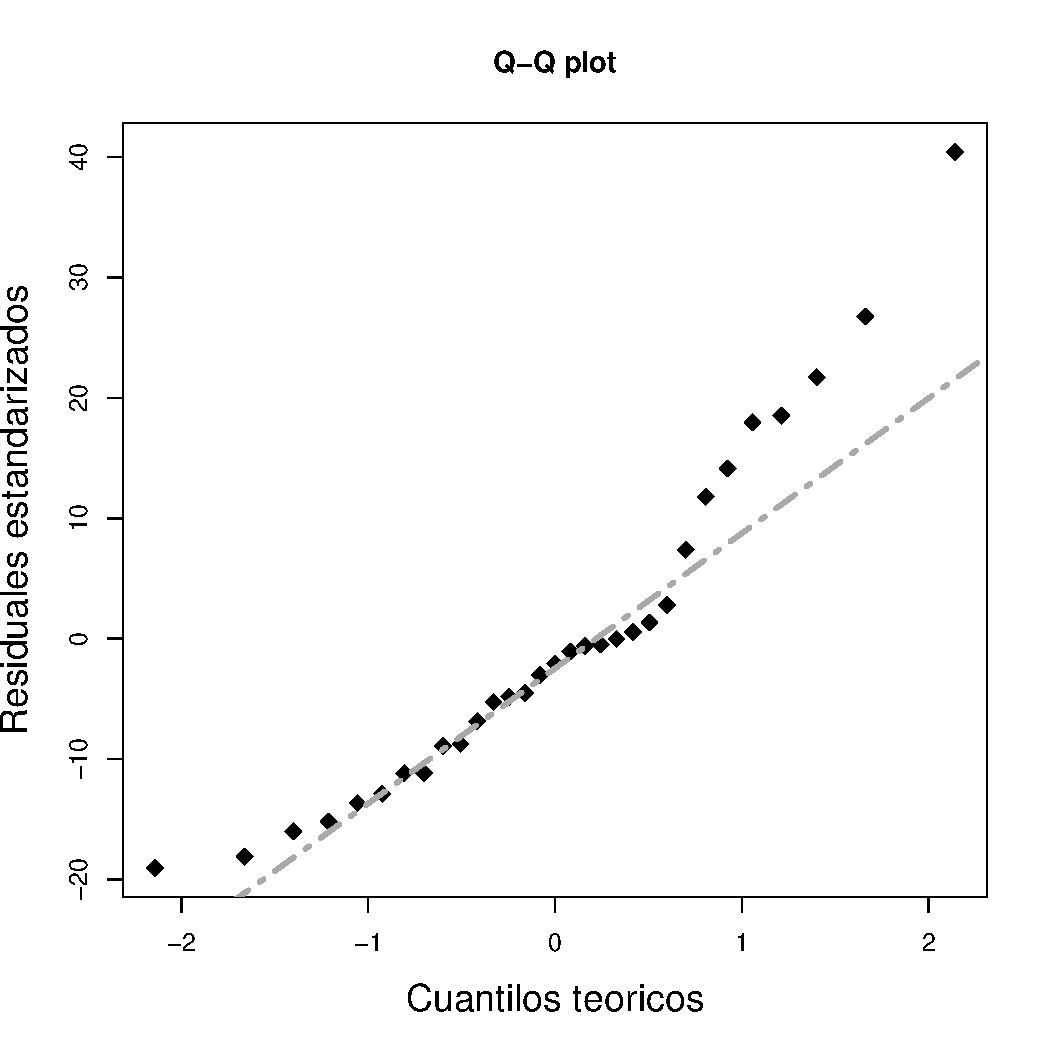
\includegraphics[scale=0.4]{figs/nonorm1.pdf}
   \end{figure}
   \vspace{-0.7cm}
   \begin{itemize}
      \item<2-| visible@2-| handout:1> Test de Shapiro-Wilk
   \end{itemize}
   \note[item]{standardized residuals = $\sqrt{MS_{residuals}}$}
\end{frame}%%%}}}


% ----- What to do when unmet assumptions? [label=assumcheck3] ----- %%{{{
\begin{frame}[label=assumcheck3]
   \frametitle{?`Qu\'e hacer si las condiciones no cumplen?}
    \begin{itemize}[<+-| visible@+-| handout:1>]
      \item Residuales no son independentes:
         \begin{itemize}
            \item[-] Modelos con efectos aleatorios (random effect models)
         \end{itemize}
      \item Residuales no son normales: 
         \begin{itemize}
            \item[-] Alternativa no par\'ametrica
            \item[-] Transformaci\'on de los datos \emph{log}, \emph{sqrt}, \emph{exp} \ldots
            \item[-] Modelo lineal generalizado (Generalized Linear Model GLM)
         \end{itemize}
      \item Heterogeneidad de la varianza:
         \begin{itemize}
            \item[-] GLM
         \end{itemize}
   \end{itemize}
\end{frame}%%%}}}

 
% ----- Inadequate model [label=modcrit2] ----- %%{{{
\begin{frame}[label=modcrit2]
   \frametitle{Si el modelo es inadecuado, se puede\ldots}
    \begin{itemize}
      \item Transformar variable dependiente
      \item Transformar $\geq1$ variable explicativa
      \item Probar otras variables explicativas
      \item Usar una estructura de error diferente (GLM)
      \item Usar alternativa no par\'ametrica (smoothing)
      \item Usar pesos diferentes por diferentes valores de $y$
   \end{itemize}
\end{frame}%%%}}}
%%}}}



% ====================== SECTION Linear regression ======================%
\section{Otros tipos de regresi\'on}

% ===== SUBSECTION:   Polynomial regression  =====%%%{{{
\subsection[Regresi\'on polinomial]{Regresi\'on polinomial}
 
% ----- Polynomial regression [label=regpol] ----- %%{{{
\begin{frame}[label=regpol]
   \frametitle{Regresi\'on polinomial}
   \framesubtitle{Ejemplo: Desintegraci\'on radioactiva}
   \begin{columns}[T, totalwidth=10cm]
      \begin{column}[]{4.6cm}
         \includegraphics<1,3-4| handout:0>[scale=0.35]{figs/polynom1.pdf}
         \includegraphics<2| handout:1>[scale=0.35]{figs/polynom2.pdf}
         \includegraphics<5| handout:2>[scale=0.35]{figs/polynom3.pdf}
         \includegraphics<6-| handout:3>[scale=0.35]{figs/polynom4.pdf}
      \end{column}
      \begin{column}[]{4.2cm}
         \begin{itemize}
            \item<2-| visible@2-| handout:1> Regresi\'on lineal: $y=ax+b$
            \item<3-| visible@3-| handout:2> Regresi\'on polin\'omica
            \item<4-| visible@4-| handout:2> $X_2=X^2$
            \item<5-| visible@5-| handout:2> $y=ax^2+bx+c$
            \item<6-| visible@6-| handout:3> $y=a \mathrm{e}^{-bx}$
            \item<7-| visible@7-| handout:3> \alert{!`Descripci\'on, no explicaci\'on!}
         \end{itemize}
      \end{column}
   \end{columns}
\end{frame}%
\note[itemize]{
   \item  probar relaci\'on no lineal pero hay que chequear si realmente describe los datos mejor o no (comparaci\'on de modelos)
   \item en este caso, cuadratica  mejor que exponencial 
   \item pero al mismo tiempo, regression exponencial hace mas sentido porque  hay chance que una curva de desintegracion no tenga un minimo
   \item tambien, es claro para todos que estos modelos son modelos lineales no cierto?
   }%%}}}
%%}}}


% ===== SUBSECTION:   Non-linear regression  =====%%%{{{
\subsection[Regresi\'on no lineal]{Regresi\'on no lineal}

% ----- Non-linear regression [label=regnolin] ----- %%{{{
\begin{frame}[label=regnolin]
   \frametitle{Regresi\'on no lineal y GAM}
   \begin{columns}[T, totalwidth=10cm]
      \begin{column}[]{4.6cm}
         \includegraphics<1-3| handout:0>[scale=0.35]{figs/regnolin1.pdf}
         \includegraphics<4-| handout:1>[scale=0.35]{figs/regnolin2.pdf}
      \end{column}
      \begin{column}[]{4.2cm}
         \begin{itemize}
            \item<2-| visible@2-| handout:1> \visible<2->{\Rlogo}: \texttt{nls()}
            \item<3-| visible@3-| handout:1> Teor\'ia: $y=a-b\mathrm{e}^{-cx}$
            \item<5-| visible@5-| handout:1> No informaci\'on: \\ Modelos Aditivos Generalizados (Generalized Additive Models GAM)
         \end{itemize}
      \end{column}
   \end{columns}
\end{frame}%%%}}}
%%}}}


% ===== SUBSECTION:   GLM  =====%%%{{{
\subsection[Modelos lineales generalizados]{Modelos lineales generalizados}
 
% ----- Generalized linear models [label=glm1] ----- %%{{{
\begin{frame}[label=glm1`]
   \frametitle{Recordatorio de vocabulario}
    \begin{itemize}
      \item Normalidad de los errores:
         \begin{itemize}
            \item[-] Modelos lineales
         \end{itemize}
      \item Normalidad + var. descriptivas continuas/categ\'oricas:
         \begin{itemize}
            \item[-] Modelos lineales generales
         \end{itemize}
      \item Errores no normales y/o varianza no homog\'enea:
         \begin{itemize}
            \item[-] Modelos lineales generalizados (GLM)
         \end{itemize}
   \end{itemize}
\end{frame}%%%}}}


% ----- Generalized linear models [label=glm2] ----- %%{{{
\begin{frame}[label=glm2]
   \frametitle{Modelos lineales generalizados (2)}
   \framesubtitle{Varianza no constante / residuales no normales}
    \begin{itemize}[<+-| handout:1>]
      \item[] \alert<.| handout:1>{$\Rightarrow$ Se puede especificar la distribuci\'on de los errores}
      \medskip
      \item<2-| handout:1> Proporciones (regresi\'on logistica) $\rightarrow$ Binomial
      \item<2-| handout:1> Conteos (modelo log-lineal) $\rightarrow$ Poisson
      \item<2-| handout:1> Variable dependiente binaria (vivo/muerto) $\rightarrow$ Binomial
      \item<2-| handout:1> Tiempo hasta muerte (varianza aumenta) $\rightarrow$ Exponencial
   \end{itemize}
\end{frame}%%%}}}
%%}}}




% ===================== SECTION Model critique ======================
\section{Criticas a los modelos}

% ----- Model criticism [label=modcrit1] ----- %%{{{
\begin{frame}[label=modcrit1]
   \frametitle{(No) enamorarse de su modelo \ldots}
    \begin{itemize}
      \item Todos los modelos son incorrectos
      \item Algunos modelos son mejores que otros
      \item El modelo correcto nunca se puede conocer con certeza
      \item Cuanto mas simple el modelo mejor
   \end{itemize}
\end{frame}%%%}}}







% =============== LECTURE/PART 4 [label=titlepart4]===============
\lecture{An\'alisis de varianza}{day4}
\part[Anova]{Anova: an\'alisis de varianza}


% ==================== SECTION:  Introduction  ====================
\section[Introducci\'on]{?`Porque no hacer multiples tests $t$?}

% ===== SUBSECTION:  Compare more than 2 samples  =====%%%{{{
\subsection[Comparar $\geq2$ muestras]{Comparar $\geq2$ muestras}

% ----- Compare 2 samples [label=anov1] ----- %%{{{
\begin{frame}[label=anov1]
   \frametitle{Comparar $\geq2$ muestras}
   \framesubtitle{Control biol\'ogico de las plagas del ma\'iz}
   \begin{exampleblock}{Ejemplo: 5 tratamientos}
      \begin{itemize}
         \item Nematodos del suelo
         \item Avispas par\'asitas
         \item Nematodos y avispas
         \item Bacterias
         \item Control
      \end{itemize}
   \end{exampleblock}
\end{frame}%%%}}}


% ----- Biological control [label=anov2] ----- %%{{{
\begin{frame}[label=anov2]
   \frametitle{Control biol\'ogico (2)}
   \begin{itemize}
      \item Muestra aleatoria por cada tratamiento
      \item Medida del peso de las mazorcas
      \item[ ] $\Rightarrow$ Media: $\mu_i$, desviaci\'on est\'andar: $\sigma_i$
      \item ?`Cu\'al tratamiento produce m\'as choclo?
      \item ?`Como comparar las medias entre tratamientos?
   \end{itemize}
\end{frame}%%%}}}
%%}}}

 
% ===== SUBSECTION:  Multiple t-tests?  =====%%%{{{
\subsection[?`Tests $t$ multiples?]{?`Hacer tests $t$ multiples?}

% ----- Why not repeated t tests ? 1 [label=anov3] ----- %%{{{
\begin{frame}[label=anov3]
   \frametitle{?`Tests $t$ repetidos?}
   \vspace{-0.5cm}
   \begin{columns}[T, totalwidth=10cm]
      \begin{column}[]{3.2cm}
         \begin{enumerate}
            \item $H_0:\mu_1=\mu_2$
            \item $H_0:\mu_1=\mu_3$
            \item $H_0:\mu_1=\mu_4$
            \item $H_0:\mu_1=\mu_5$
            \item $H_0:\mu_2=\mu_3$
            \item $H_0:\mu_2=\mu_4$
            \item $H_0:\mu_2=\mu_5$
            \item $H_0:\mu_3=\mu_4$
            \item $H_0:\mu_3=\mu_6$
            \item $H_0:\mu_4=\mu_5$
         \end{enumerate}
      \end{column}
      \visible<1-| handout:1>{\begin{column}[]{6.5cm}
         \begin{itemize}[<+-| visible@+-| handout:1>]
            \item Cada hip\'otesis: riesgo de error de tipo I
            \item Con 1 hip\'otesis: $\alpha = 0.05$
            \item ?`Valor de $\alpha$ con 2 hip\'otesis?
            \item ?`$0.025$, $0.05$, $0.0725$, $0.0975$, $0.10$?
            \item $1-Pr(no~error~de~tipo~I)$
            \item $1-0.95\cdot0.95=\alert<.| handout:1>{0.0975}$
         \end{itemize}
      \end{column}
      }
   \end{columns}
\end{frame}%%%}}}


% ----- Why not repeated t-tests 2 [label=anov4] ----- %%{{{
\begin{frame}[label=anov4]
   \frametitle{?`Tests $t$ repetidos?}
   \framesubtitle{!`Amplifica el riesgo de error de tipo I!}

   \footnotesize

   \begin{table}
      \begin{tabular}{ccc}
         \firsthline
         \\[-0.85cm]
         \parbox[t]{13ex}{\flushleft n\'umero de muestras $i$} & \parbox[t]{13ex}{\flushleft n\'umero de hip\'otesis $j$} & \parbox[t]{13ex}{\flushleft Riesgo total $1-0.95^j$} \\
         \\[-1ex]
         \hline \\[-1ex]
         2 & 1 & 0.05 \\
         3 & 3 & 0.14 \\
         4 & 6 & 0.26 \\
         \alert{5} & \alert{10} & \alert{0.40} \\
         6 & 15 & 0.54 \\
         10 & 45 & 0.90 \\
         \lasthline
      \end{tabular}
   \end{table}
\end{frame}%%%}}}


% ----- Why not repeated t-tests? 3 [label=anov5] ----- %%{{{
\begin{frame}[label=anov5]
   \frametitle{El problema con tests $t$ multiples}
    \begin{itemize}
      \item Riesgo de error de tipo I m\'as grande
      \item Solo considera variaci\'on para 2 muestras al mismo tiempo $\Rightarrow$ precisi\'on baja
      \item No es posible considerar estructuras complicadas (\emph{e.g.} 2 factores experimentales)
      \medskip
      \item[ ] $\Rightarrow$ El an\'alisis de varianza se encarga de estos problemas
   \end{itemize}
\end{frame}%%%}}}
%%}}}



% ==================== SECTION:  Anova: definition  ====================%
\section[Definici\'on]{?`Qu\' es el anova?}

% ===== SUBSECTION:  Concept of anova  =====%%%{{{
\subsection[Concepto]{Concepto del Anova}
 
% ----- Anova concept [label=anov6] ----- %%{{{
\begin{frame}[label=anov6]
   \frametitle{Concepto del Anova}
    \begin{itemize}[<+-| handout:1>]
      \item Variables explicativas categ\'oricas = \alert{factores}
      \item $\geq 2$ \alert{niveles} / grupos / tratamientos
      \item Dividir entre variaci\'on \structure<.| handout:1>{no explicada} y variaci\'on \structure<.>{explicada} por las variables explicativas
      \item Ajustar modelos lineales para \structure<.| handout:1>{explicar} o \structure<.>{predecir} valores de la variable dependiente
   \end{itemize}
\end{frame}%%%}}}
%%}}}


% ===== SUBSECTION:  Objectives of anova  =====%%%{{{
\subsection[Objetivos]{Objetivos del Anova}

% ----- Objectives of the Anova [label=anov7] ----- %%{{{
\begin{frame}[label=anov7]
   \frametitle{Objetivos del Anova}
    \begin{itemize}[<+-| handout:1>]
      \item Examinar la contribuci\'on relativa de diferentes fuentes de variaci\'on sobre la cantidad total de variaci\'on de la variable dependiente
      \item Evaluar la hip\'otesis $H_0$ que las medias de los grupos / tratamientos son iguales
   \end{itemize}
\end{frame}%%%}}}
%%}}}


% ===== SUBSECTION:  Various types of anova  =====%%%{{{
\subsection[Varios tipos]{Varios tipos de Anova}
 
% ----- Various types of anova [label=anov8] ----- %%{{{
\begin{frame}[label=anov8]
   \frametitle{Varios tipos de anova}
    \begin{itemize}[<+-| handout:1>]
      \item 1 factor, 2 niveles $\rightarrow$ test $t$
      \item 1 factor, $\geq 3$ niveles $\rightarrow$ anova simple (one-way anova)
      \item $\geq 2$ factores $\rightarrow$ anova de 2 or 3 factores (two/three-way anova)
      \item Replicaci\'on por cada nivel $\rightarrow$ dise\~no factorial $\Rightarrow$ permite estudiar las interacciones entre variables
   \end{itemize}
\end{frame}%%%}}}
%%}}}



% ==================== SECTION:  Anova: principle  ====================%
\section[Anova simple]{Principio del anova simple}

% ===== SUBSECTION:  Worked example  =====%%%{{{
\subsection[Ejemplo: ozono]{Ejemplo: concentraci\'on de ozono}

% ----- Analysis of variance to compare means [label=anov9] ----- %%{{{
\begin{frame}[label=anov9]
   \frametitle{An\'alisis de varianza ?`para comparar medias?}
   \begin{exampleblock}{Ejemplo: Cantidad de ozono}
      \begin{itemize}
         \item Variable dependiente $Y$: concentraci\'on de ozono
         \item Variable explicativa: 1 factor \textsc{Jard\'in}, 2 niveles $A$ y $B$
         \item 10 r\'eplicas por jard\'in
         \medskip
         \item ?`La concentraci\'on de  ozono es la misma?
      \end{itemize}
   \end{exampleblock}
\end{frame}%%%}}}
%%}}}


% ===== SUBSECTION:  Principle of anova  =====%%%{{{
\subsection[Principio]{Principio del Anova}

% ----- Principle of Anova 1 [label=anov10] ----- %%{{{
\begin{frame}[label=anov10,plain]
   \frametitle{Principio del Anova (1)}
   \vspace{-0.5cm}
   \begin{columns}[c, totalwidth=10cm]
      \hspace{-1.5cm}
      \begin{column}[]{5.5cm}
         \includegraphics<1-2| handout:0>[scale=0.6]{figs/principANOV1.png}
         \includegraphics<3| handout:0>[scale=0.6]{figs/principANOV2.png}
         \includegraphics<4-| handout:1>[scale=0.6]{figs/principANOV3.png}
      \end{column}
      \begin{column}[]{5cm}
         \begin{itemize}
            \item<2-| visible@2-| handout:1> Mucha dispersi\'on 
            \item<3-| visible@3-| handout:1> Concentraci\'on media
            \smallskip
            \item<4-| visible@4-| handout:1> $\visible<7->{SSY=}\visible<6->{\sum}\visible<5->{(}y_i-\bar{y}\visible<5->{)^2}$
            \smallskip
            \item<7-| visible@7-| handout:1> \alert<7>{Residuales}: suma total de los cuadrados (total sum of squares SSY)
            \item<8-| visible@8-| handout:1> Variaci\'on \alert{entre} los tratamientos
         \end{itemize}
      \end{column}
   \end{columns}
\end{frame}%%%}}}

  
% ----- Principle of Anova 2 [label=anov11] ----- %%{{{
\begin{frame}[label=anov11,plain]
   \frametitle{Principio del Anova (2)}
   \vspace{-0.5cm}
   \begin{columns}[c, totalwidth=10cm]
      \hspace{-1.5cm}
      \begin{column}[]{5.5cm}
         \includegraphics<1| handout:0>[scale=0.6]{figs/principANOV4.png}
         \includegraphics<2| handout:0>[scale=0.6]{figs/principANOV5.png}
         \includegraphics<3-| handout:1>[scale=0.6]{figs/principANOV6.png}
      \end{column}
      \begin{column}[]{5cm}
         \begin{itemize}[<+-| visible+-| handout:1>]
            \item<1-| visible@1-| handout:1> Jard\'in $A$
            \item<3-| visible@3-| handout:1> Jard\'in $B$
            \item<4-| visible@4-| handout:1> $C_B>C_A$
            \item<5-| visible@5-| handout:1> ?`La diferencia es significativa o no?
         \end{itemize}
      \end{column}
   \end{columns}
\end{frame}%%%}}}

  
% ----- Principle of Anova 3 [label=anov12] ----- %%{{{
\begin{frame}[label=anov12,plain]
   \frametitle{Principio del Anova (3)}
   \vspace{-0.5cm}
   \begin{columns}[c, totalwidth=10cm]
   \hspace{-1.5cm}
      \begin{column}[]{5.5cm}
         \includegraphics<1,3| handout:0>[scale=0.6]{figs/principANOV6.png}
         \includegraphics<2| handout:1>[scale=0.6]{figs/principANOV3.png}
         \includegraphics<4| handout:0>[scale=0.6]{figs/principANOV9.png}
         \includegraphics<5| handout:0>[scale=0.6]{figs/principANOV7.png}
         \includegraphics<6-8| handout:0>[scale=0.6]{figs/principANOV7.png}
         \includegraphics<9| handout:2>[scale=0.6]{figs/principANOV8.png}
      \end{column}
      \begin{column}[]{5cm}
         \begin{itemize}[<+-| visible@+-| handout:1>]
         \item<1-| visible@1-| handout:1>?`Qu\'e pasa con los residuales si $\bar{y}_{_A}=\bar{y}_{_B}$?
         \item<3-| visible@3-| handout:2>?`Y si \alert<9->{$\bar{y}_{_A}\neq \bar{y}_{_B}$}?
         \medskip
         \item<4-| visible@4-| handout:2> \small{$ \visible<5->{SSE = \sum_{j=1}^{k}}\visible<4->{\sum(y_{ij}-\bar{y}_j)^2} $}
         \medskip
         \item<6-| visible@6-| handout:2> Suma de cuadrados del error (Error sum of squares SSE)
         \item<7-| visible@7-| handout:2> Variaci\'on \alert<5>{dentro} de los tratamientos
         \item<8-| visible@8-| handout:2> \alert<6>{?`$SSE$ versus $SSY$ ?}
         \item<9-| visible@9-| handout:2> \alert{!`$SSE<SSY$!}
         \end{itemize}
      \end{column}
   \end{columns}
\end{frame}%%}}}
%%}}}


% ===== SUBSECTION:  Worked example summary of principle  =====%%%{{{
\subsection[Resumen]{Resumen del principio del anova}
 
% ----- Summary Principle of Anova [label=anov13] ----- %%{{{
\begin{frame}[label=anov13]
   \frametitle{Para resumir}
   \framesubtitle{An\'alisis de varianza para comparar medias}
    \begin{itemize}
      \item<1-| visible@1-| handout:1> Cuando $\bar{y}_{_A}\neq \bar{y}_{_B}$, $SSE < SSY$
      \item<2-| visible@2-| handout:1> Variaci\'on total = modelo + error
      \item<3-| visible@3-| handout:1> $SSY = SSA+SSE$
      \item<4-| visible@4-| handout:1> $SSA$: proporci\'on de varianza explicada 
      \item<5-| visible@5-| handout:1> Si $SSE<SSY \Rightarrow \bar{y}_A\neq\bar{y}_B$
   \end{itemize}
\end{frame}%%%}}}
%%}}}


% ===== SUBSECTION:  Worked example back to the garden  =====%%%{{{
\subsection[En el jard\'in]{De vuelta al jard\'in}
 
% ----- Back to the garden [label=anov15] ----- %%{{{
\begin{frame}[label=anov15]
   \frametitle{De vuelta al jard\'in \ldots}
    \begin{itemize}
      \item $SSY=44$
      \item ?`Cuanto es atribuible a la diferencia entre $\bar{y}_{_A}$ y $\bar{y}_{_B}$?
      \item Jard\'in $A$: $SSE_A=12$, Jard\'in $B$: $SSE_B=12$
      \item Suma de cuadrados de error $SSE=SSE_A+SSE_B=12+12=24$
      \item Suma de cuadrados del tratamiento: $SSA=SSY-SSE=44-24=20$
   \end{itemize}
\end{frame}%%%}}}
%%}}}


% ===== SUBSECTION:  the anova table  =====%%%{{{
\subsection[Tabla de anova]{Tabla de anova}

% ----- Anova table [label=anov16] ----- %%{{{
\begin{frame}[label=anov16]
   \frametitle{Tabla de Anova}
   \small
   \renewcommand{\arraystretch}{1.3}
   \begin{table}
      \begin{tabular}{ccccc}
         \firsthline
         \\[-2ex]
         \parbox[c]{9ex}{\centering Fuente} & \parbox[c]{10ex}{\centering Suma de cuadrados} & \parbox[c]{10ex}{\centering Grados de libertad} & \parbox[c]{9ex}{\centering Cuadrado medio} & \parbox[c]{9ex}{\centering Raz\'on-F} \\[2ex]
         \hline
         Jard\'in & $SSA=20.0$ & $1 $ & $20.0$         & $15.0$ \\
         Error    & $SSE=24.0$ & $18$ & $s^2=1.33$ &      \\
         Total    & $SSY=44.0$ & $19$ &              &      \\
         \lasthline
      \end{tabular}
   \end{table}

   \begin{itemize}[<2-| visible@+(1)-| handout:1>]
      \item $F_{teo}=4.41$, ?`Qu\'e se puede concluir?
      \item No se puede aceptar $H_0$
      \item $\bar{y}_{_A}\neq\bar{y}_{_B}$
      \item Concentraci\'on de ozono es diferente entre los jardines $A$ y $B$
   \end{itemize}
   \note[item]{antes de concluir, me pueden recordar la hipotesis nula?}
\end{frame}%%%}}}
%%}}}


% ===== SUBSECTION:  assumptions of anova  =====%%%{{{
\subsection[Condiciones]{Condiciones del anova}

% ----- Assumptions of anova [label=anovacond] ----- %%{{{
\begin{frame}[label=anovcond]
   \frametitle{Condiciones del anova}
   \framesubtitle{!`Las mismas que por la regresi\'on!}
    \begin{itemize}
      \item Independencia
      \item Homogeneidad de las varianzas
      \item Normalidad
      \medskip
      \item[] !`Condiciones sobre los residuales! $\Rightarrow$ hacer los tests despues del an\'alisis
   \end{itemize}
\end{frame}%%%}}}
%%}}}



% ==================== SECTION:  More complex designs  ====================%
\section[Otros dise\~nos]{Dise\~nos m\'as complejos}

% ===== SUBSECTION:  factorial designs  =====%%%{{{
\subsection[Dise\~no factorial]{Dise\~no factorial}

% ----- Factorial experiment [label=factexp] ----- %%{{{
\begin{frame}[label=factexp]
   \frametitle{Dise\~nos factoriales}
    \begin{itemize}
      \item $\geq2$ factores
      \item $\geq2$ niveles per factor
      \item Replicaci\'on para cada combinaci\'on de niveles
      \item Interacciones: respuesta a un factor depende del nivel de otro factor
   \end{itemize}
\end{frame}%%%}}}


% ----- Nested design - split plot [label=nestsplit] -----  %%{{{
\begin{frame}[label=nestsplit]
   \frametitle{Reconocer dise\~nos complicados para evitar seudoreplicaci\'on} 
   \framesubtitle{(Nested design and Split plots)} 
   \begin{itemize} 
      \item \structure{Muestreo jer\'arquico}: medidas repetidas del mismo individuo o estudios con varias escalas espaciales 
      \item \structure{Parcelas subdivididas}: diferentes tratamientos en diferentes parcelas de diferentes tama\~nos
      \end{itemize}
   \note[item]{estos disenos permiten tener estructuras de errores complicadas}
\end{frame}%%%}}}

 
% ----- Split plot example  [label=splitploteg] ----- %%{{{
\begin{frame}[label=splitploteg]
   \frametitle{Un ejemplo de dise\~no ``split plot''}
   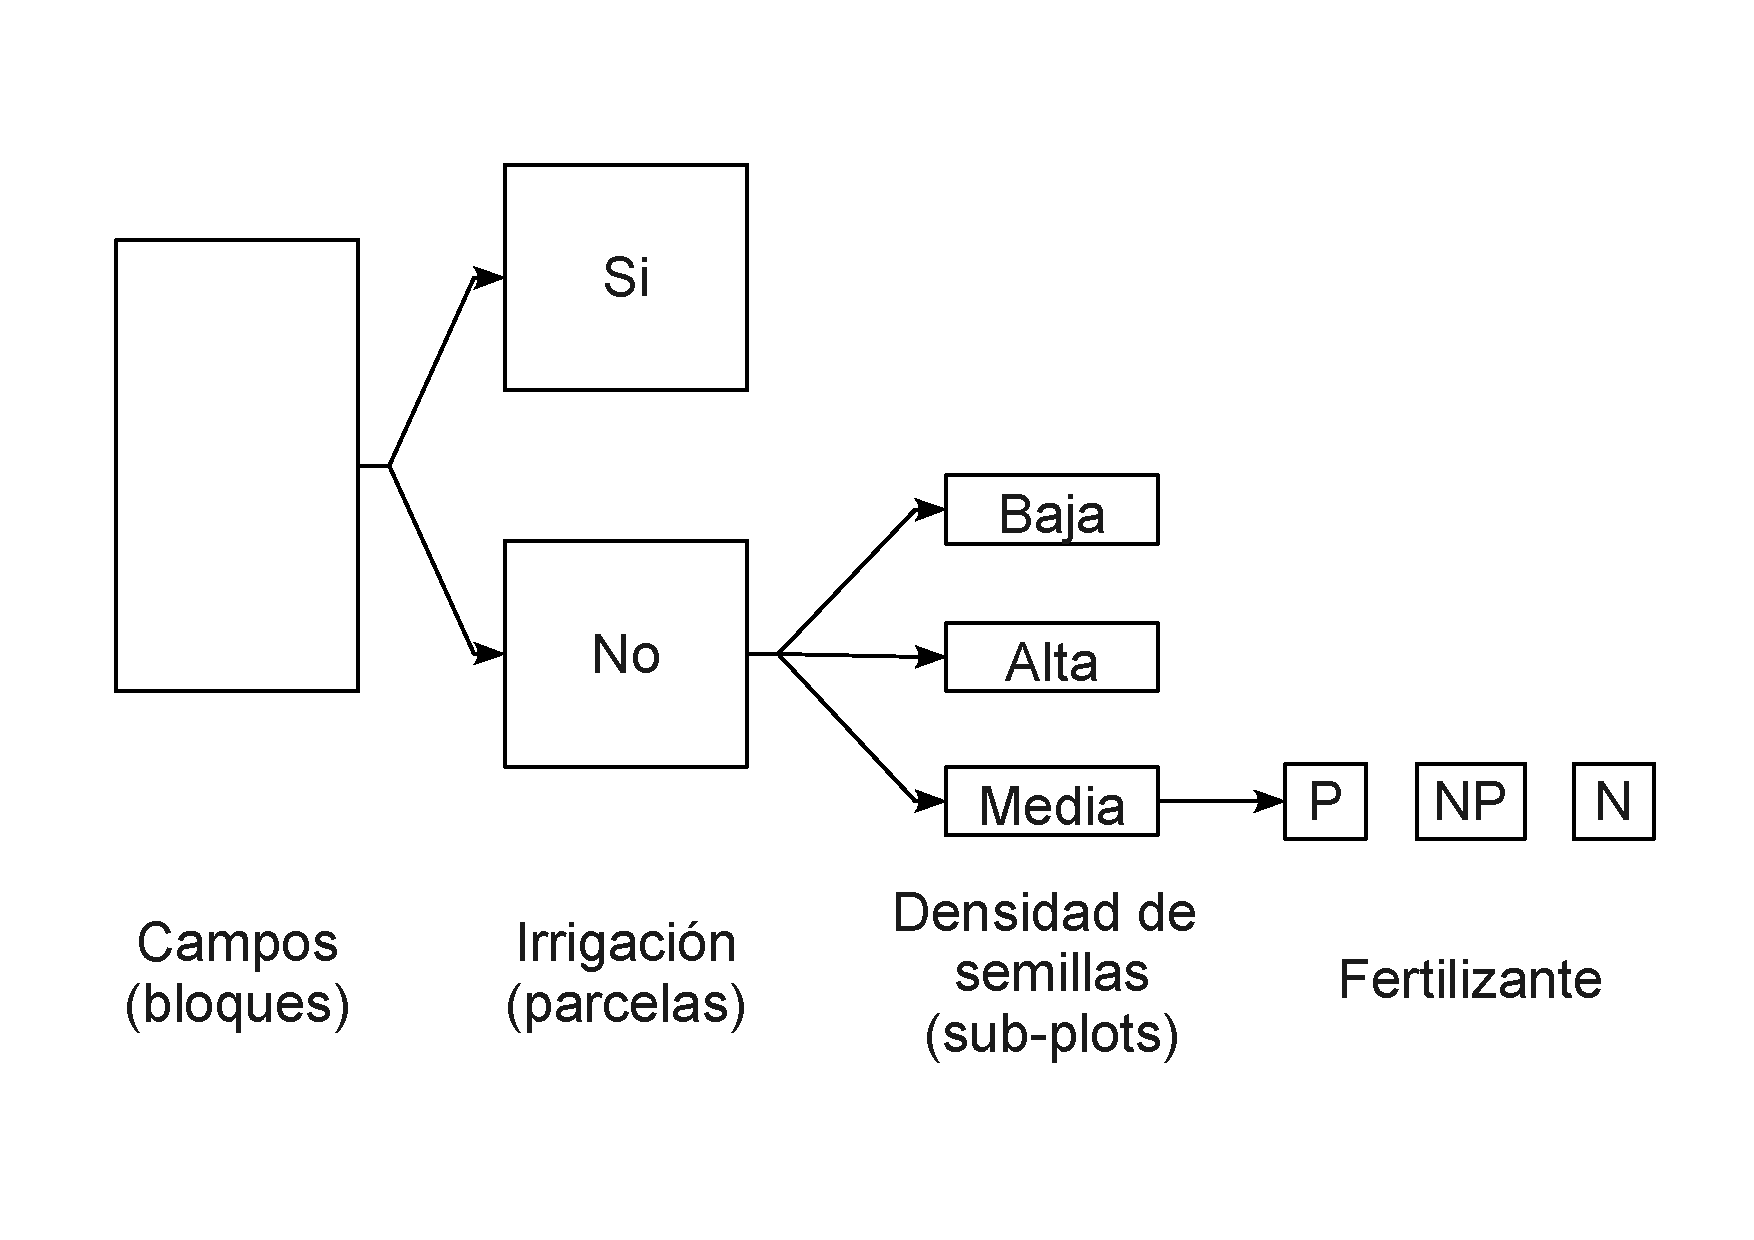
\includegraphics[scale=0.35]{figs/splitplot.pdf}
\end{frame}%%%}}}
%%}}}


% ===== SUBSECTION:  Types of factors  =====%%%{{{
\subsection[Tipos de factores]{Tipos de factores}

% ----- Types of variables [label=typesvar1] ----- %%{{{
\begin{frame}[label=encours]
   \frametitle{Factores fijos}
   \framesubtitle{(Fixed effects)}
   \begin{itemize}
      \item Todos los niveles estan incluidos
      \item No extrapolaci\'on fuera de estos niveles
      \item Si se repite el estudio $\rightarrow$ mismos niveles
      \item Modelos con efectos fijos (fixed effects models)
      \item Anova tipo I
      \item Ejemplo: nivel de zinc (Fondo, bajo, medio alto), fertilizantes \ldots
   \end{itemize}
\end{frame}%%%}}}

 
% ----- Types of variables 2 [label=typesvar2] ----- %%{{{
\begin{frame}[label=encours]
   \frametitle{Factores aleatorios}
   \framesubtitle{(Random effects)}
    \begin{itemize}
         \item Muestra aleatoria de los niveles posibles
         \item Inferencia (extrapolaci\'on) sobre todos los grupos
         \item Si se repite el estudio $\rightarrow$ otros niveles
         \item Modelos de efectos aleatorios (random effect models)
         \item Anova tipo II
         \item Ejemplo: Sitios de estudio, \ldots
   \end{itemize}
\end{frame}%%%}}}
%%}}}


\end{document}














